\documentclass[12pt,a4paper]{article}

\usepackage[utf8]{inputenc}
\usepackage[T1]{fontenc}
\usepackage{lmodern}
\usepackage{amsmath,amssymb,amsfonts}
\usepackage{amsthm}
\usepackage{graphicx}
\usepackage{booktabs}
\usepackage{array}
\usepackage{tabularx}
\usepackage{ragged2e}
\usepackage{hyperref}
\usepackage{geometry}
\usepackage{xcolor}
\usepackage{enumitem}
\usepackage{caption}
\usepackage{float}
\usepackage{url}
\usepackage{microtype}
\usepackage{setspace}
\usepackage{fancyhdr}
\usepackage{algorithm}
\usepackage{algpseudocode}
\usepackage{appendix}
\usepackage{tocloft}
\usepackage{tikz}
\usetikzlibrary{arrows.meta,positioning,calc,fit}
\usepackage{pgfplots}
\pgfplotsset{compat=1.17}
\pgfplotsset{every axis/.append style={font=\footnotesize}}

\setcounter{tocdepth}{2}
\renewcommand{\cftbeforesecskip}{3pt}
\setlength{\cftparskip}{0pt}
\setlength{\cftsubsecindent}{1.5em}
\setlength{\cftsecindent}{0em}

\geometry{a4paper, margin=2.5cm}

\linespread{1.08}
\setlength{\headheight}{14pt}
\emergencystretch=2em
\setlength{\parskip}{3pt}

\setlength{\aboverulesep}{2.5pt}
\setlength{\belowrulesep}{2.5pt}
\setlength{\extrarowheight}{2pt}

\captionsetup{font=small, labelfont=bf, textfont=it, skip=6pt}

\hypersetup{
    colorlinks=true,
    linkcolor=blue!70!black,
    citecolor=blue!70!black,
    urlcolor=blue!70!black,
    pdftitle={UniMind: A Middleware Framework for Bridging Classical AI Workloads and Quantum Computing Backends},
    pdfauthor={Y. X. Tan}
}

\newtheorem{definition}{Definition}[section]

\pagestyle{fancy}
\fancyhf{}
\fancyhead[L]{\small\itshape UniMind: A Middleware Framework}
\fancyhead[R]{\small\thepage}
\renewcommand{\headrulewidth}{0.4pt}

\floatname{algorithm}{Algorithm}

\newcommand{\umcheck}{\checkmark}
\newcommand{\umcross}{$\times$}

\begin{document}

\begin{titlepage}
\centering
\vspace*{2cm}

{\LARGE\bfseries UniMind: A Middleware Framework for\\[6pt]
Bridging Classical AI Workloads and\\[6pt]
Quantum Computing Backends\par}

\vspace{0.8cm}

{\normalsize\rmfamily Version 2.5 (August 30, 2026) --- 7-dim $J(G)$ with $E_{\rm 2q\_log}$/$E_{\rm idle}$, 150-iter Pareto frontier, calibration-weighted SABRE v3\par}

\vspace{1.2cm}

{\Large Y. X. Tan\par}
\vspace{0.3cm}
{\normalsize\itshape Independent Researcher\par}
{\normalsize\itshape Email: yxtan5022@gmail.com\par}

\vspace{1.8cm}

{\large\bfseries Abstract\par}
\vspace{0.5cm}

\begin{minipage}{0.92\textwidth}
\small
As quantum computing transitions from theoretical research to practical deployment, a compatibility gap emerges between classical AI software stacks and probabilistic quantum hardware. Existing quantum machine learning frameworks operate at the application level and lack system-level abstractions for hardware adaptation, workload routing, and dynamic code generation. This paper presents \textbf{UniMind}, a middleware framework designed to reduce the abstraction gap between classical AI workloads and heterogeneous quantum-classical computing backends. UniMind introduces two components: (1)~an \textbf{LLM-driven orchestration layer} that interprets high-level task specifications and generates topology-aware execution plans through constrained sampling, operating exclusively in user space with sandboxed validation and rule-based fallback; and (2)~\textbf{Unibit}, a classical preprocessing representation based on sliding-window frequency estimation and sinc-based smoothing that produces parameters for standard quantum angle encoding. We implement a multi-backend mapping engine and validate the framework with reproducible experiments: mathematical correctness (empirical measurement probabilities converge to theoretical weights across 8192 shots, maximum $\langle Z \rangle$ deviation of $0.0110$), system performance (up to $10.9\times$ speedup via vectorized C-backend execution and $4.5\times$ end-to-end speedup via the Rust FFI engine, with a component-level breakdown attributing the residual overhead to Python-side normalization and marshaling), a three-arm baseline comparison against bare Qiskit and a rule-based dispatcher (only the UniMind pipeline covers all five benchmark task classes), an LLM-reliability benchmark (success rate 91.7--100\% across injected LLM quality levels, measured at $n{=}200$ per level with Wilson confidence intervals, with $100\%$ rejection of all adversarial intents), fault-injection analysis (four of five fault classes recovered in sub-millisecond detection time; one exposes a real robustness gap), a noise-sensitivity analysis quantifying the encoding's degradation under depolarizing and $T_1$ channels, a sandbox security evaluation (20 of 21 escape attempts blocked), and physical QPU validation on IBM hardware (\texttt{ibm\_marrakesh}): a placement-controlled QPU sweep on \texttt{ibm\_marrakesh} in which the bare encoding meets the $0.05$ tolerance across weights $w \in [0.05, 0.95]$ when the layout is pinned to a well-calibrated qubit (maximum $\langle Z \rangle$ deviation $0.028$), while an adversarially chosen qubit with $82\%$ readout error inflates distortion to $0.213$ --- establishing that single-qubit encoding fidelity on real hardware is dominated by placement and calibration state rather than by the encoding itself, with a two-parameter affine channel model $P_{\mathrm{obs}} = b + a\,w$ fitting every condition at shot-noise level; a component ablation attributing up to $+34$ points of success rate to the self-healing layer and showing that rule-based fallback reaches $100\%$ recovery under availability stress once template coverage is complete; and a path-decomposition calculus whose exact absorbing-chain model (validated on all 23 testable cells) shows that the apparent gap between naive independence predictions and measured healing rates is a retry-budget truncation effect, not stochastic correlation; a calibration-scored hardware-routing study in which a zero-fit readout-error score $C(q)$, evaluated over all 156 qubits of \texttt{ibm\_marrakesh}, selects layouts at sub-millisecond overhead but whose strict monotone ranking did not survive replication ($\rho_s = 1.000$ on the initial snapshot; $0.771$, $p = 0.103$ on the fixed-design re-run, hypothesis H3.1 unvalidated); and an end-to-end composition experiment in which the full pipeline (full-coverage fallback + calibration-aware placement) completes $54/54$ orchestrated tasks ($100\%$) versus $87.0\%$ for the stage-ablated pipeline; the quantum-fidelity leg, measured at 30 angle-encoding circuits per arm under a frozen two-day-old calibration, shows \emph{no} calibration-placement advantage at the $0.05$ tolerance ($36.7\%$ vs.\ $40.0\%$ pass, overlapping Wilson intervals) --- a null result consistent with the routing replication and the quantified cross-day calibration drift, and therefore reported without overclaiming. We discuss the remaining limitations---notably deeper hardware error mitigation and cross-framework comparison---and propose a phased roadmap for quantum-ready AI middleware.
\end{minipage}

\vspace{0.8cm}

\noindent\textbf{Keywords:} Quantum Computing, AI Middleware, Angle Encoding, Hybrid Quantum-Classical Systems, LLM Orchestration, Unibit

\vfill

{\small\copyright\ 2026 Y. X. Tan. This work is licensed under CC BY 4.0; the accompanying software (\texttt{unimind-os}) is MIT-licensed.}

\vspace{0.4cm}

{\small\itshape Name-disambiguation note: the name ``UniMind'' is also used by an unrelated prior work on LLM-based multi-task brain decoding~\cite{lu2025unimind}; the present work is not affiliated with that work.\par}

\end{titlepage}

\tableofcontents
\newpage

\section{Introduction}

The rapid advancement of quantum computing hardware has introduced a growing mismatch between the capabilities of emerging quantum processors and the software infrastructure available to utilize them. Modern AI systems---deep learning models, reinforcement learning agents, and large language models---are built upon software stacks designed for deterministic, von Neumann architectures. Operating systems such as Linux, Windows, and macOS manage discrete binary states through priority-based schedulers, static device drivers, and predictable memory hierarchies~\cite{tanenbaum2023}. These assumptions are fundamentally incompatible with the probabilistic, measurement-driven execution model of quantum computers.

Current approaches to quantum machine learning (QML), including frameworks such as PennyLane~\cite{bergholm2018}, TensorFlow Quantum, and Qiskit Machine Learning, provide algorithm-level abstractions for constructing and training quantum circuits. However, these frameworks operate within existing classical operating systems and do not address system-level challenges such as dynamic hardware discovery, workload routing across heterogeneous backends, or intent-driven task orchestration. As quantum hardware diversifies---spanning superconducting qubits, trapped ions, photonic systems, and GPU-accelerated simulators~\cite{microsoft2024,aws2024}---the need for a unified middleware layer becomes increasingly apparent.

This paper presents \textbf{UniMind}, a middleware framework that addresses this gap. UniMind is not an operating system; it operates as a user-space orchestration layer atop existing classical operating systems. Its design is motivated by three observations:

\begin{enumerate}[leftmargin=2em]
    \item \textbf{Hardware heterogeneity is increasing.} AI workloads must increasingly target diverse backends (CPUs, GPUs, QPUs, simulators), each with distinct programming models and performance characteristics.
    \item \textbf{Intent-driven computing is emerging.} Large language models can translate natural language specifications into executable code, potentially reducing the barrier to programming heterogeneous systems~\cite{wang2024}.
    \item \textbf{Classical-to-quantum data encoding remains manual.} Translating classical data into quantum states typically requires hand-crafted encoding circuits, creating friction in hybrid workflows.
\end{enumerate}

UniMind addresses these observations through three components:

\begin{itemize}
    \item An \textbf{LLM-driven orchestration layer} (Section~\ref{sec:orchestrator}) that interprets task specifications and generates execution plans, subject to sandboxed validation and deterministic fallback mechanisms.
    \item \textbf{Unibit} (Section~\ref{sec:unibit}), a classical preprocessing representation that computes sliding-window frequency estimates over binary sequences, producing parameters suitable for standard quantum angle encoding.
    \item A \textbf{multi-backend quantum mapping engine} (Section~\ref{sec:bridge}) that translates Unibit parameters into parameterized quantum circuits and routes execution to available backends.
\end{itemize}

The main contributions of this paper are:

\begin{enumerate}[leftmargin=2em]
    \item We identify system-level gaps between classical AI software stacks and quantum computing hardware that are not addressed by existing QML frameworks.
    \item We propose UniMind, a middleware framework with an LLM-driven orchestration layer, a classical preprocessing representation (Unibit), and a multi-backend quantum mapping engine.
    \item We present a functional proof-of-concept implementation in C++, Rust, and Python, with \textbf{quantitative validation}: mathematical verification via 8192-shot measurement convergence ($\langle Z \rangle$ deviation $= 0.0110$), performance micro-benchmarks demonstrating up to $10.9\times$ speedup via vectorized C-backend execution and $4.5\times$ end-to-end speedup via Rust FFI (with a component-level latency breakdown), a three-arm baseline comparison, an LLM-reliability benchmark, fault-injection analysis, a noise-sensitivity study, a sandbox security evaluation, and placement-controlled physical QPU sweeps on \texttt{ibm\_marrakesh} (bare encoding within tolerance on calibrated layouts, max.\ deviation $0.028$; adversarial placement inflates distortion to $0.213$), an architectural ablation, an instrumented failure taxonomy, an exact reliability-composition calculus validated on all 23 testable cells, a calibration-scored routing study whose initial perfect rank correlation ($\rho_s = 1.000$) did not replicate on a fixed-design re-run ($\rho_s = 0.771$, $p = 0.103$) and is reported without overclaiming, and an end-to-end composition experiment separating software-path reliability ($100\%$ vs.\ $87.0\%$) from hardware fidelity.
    \item We provide an honest, experiment-backed assessment of limitations---including LLM reliability, quantum noise sensitivity, and the security of LLM-generated code---and outline the experiments still required for future validation.
    \item We propose a phased roadmap for the development of quantum-ready AI middleware.
\end{enumerate}

\paragraph{Scope and limitations.} This paper presents a system design and proof-of-concept implementation. We do not claim quantum advantage, novel quantum algorithms, or comprehensive end-to-end system evaluation. The Unibit-to-qubit mapping is an instance of standard angle encoding~\cite{schuld2021}; our contribution lies in the classical preprocessing pipeline and the multi-backend orchestration layer, not in the quantum circuit design itself.

The remainder of this paper is organized as follows. Section~\ref{sec:background} provides background. Section~\ref{sec:architecture} presents the UniMind architecture. Section~\ref{sec:implementation} describes the implementation. Section~\ref{sec:evaluation} presents quantitative evaluation with real experimental data. Section~\ref{sec:discussion} discusses limitations, threats to validity, and a roadmap. Section~\ref{sec:conclusion} concludes.


\section{Background}\label{sec:background}

\subsection{Classical Operating Systems and AI}

Modern operating systems are designed around the von Neumann architecture, where a central processing unit sequentially fetches, decodes, and executes instructions from memory~\cite{tanenbaum2023}. The OS kernel manages hardware resources through device drivers, process schedulers, and memory managers, providing a stable abstraction layer for user-space applications.

AI workloads, particularly deep learning, operate within this paradigm. Neural networks are represented as computational graphs of matrix multiplications and nonlinear activations, executed on CPUs, GPUs, or specialized accelerators. The software stack assumes deterministic, sequential execution with well-defined memory addresses.

This paradigm presents three limitations for quantum-era computing:

\begin{enumerate}[leftmargin=2em]
    \item \textbf{Binary rigidity.} Classical bits exist in exactly one of two states (0 or 1), whereas quantum computation manipulates continuous probability amplitudes.
    \item \textbf{Deterministic scheduling.} Classical OS schedulers assume predictable execution times, incompatible with probabilistic, shot-based quantum execution.
    \item \textbf{Static hardware abstraction.} Traditional device drivers cannot dynamically adapt to heterogeneous quantum-classical hybrid systems.
\end{enumerate}

\subsection{Quantum Computing Fundamentals}

Quantum computing leverages quantum mechanical principles to process information. The fundamental unit is the \textbf{qubit}:
\begin{equation}
    |\psi\rangle = \alpha|0\rangle + \beta|1\rangle
\end{equation}
where $\alpha, \beta \in \mathbb{C}$ satisfy $|\alpha|^2 + |\beta|^2 = 1$.

Quantum operations are performed through \textbf{quantum gates}. Key gates include:
\begin{itemize}
    \item \textbf{Pauli-X gate:} $X = \begin{pmatrix} 0 & 1 \\ 1 & 0 \end{pmatrix}$ (bit flip)
    \item \textbf{Y-rotation gate:} $R_y(\theta) = \begin{pmatrix} \cos(\theta/2) & -\sin(\theta/2) \\ \sin(\theta/2) & \cos(\theta/2) \end{pmatrix}$
    \item \textbf{Hadamard gate:} $H = \frac{1}{\sqrt{2}}\begin{pmatrix} 1 & 1 \\ 1 & -1 \end{pmatrix}$
\end{itemize}

A quantum circuit applies a sequence of gates to a qubit register, followed by measurement that collapses the state into classical bits according to the Born rule.

Current hardware operates in the \textbf{NISQ} era~\cite{preskill2018}, characterized by 50--1000 qubits, high gate error rates, and short coherence times. Prominent quantum algorithms include Shor's factoring algorithm~\cite{shor1994} and variational quantum eigensolvers~\cite{kandala2017}, and quantum machine learning has been surveyed extensively~\cite{biamonte2017,cerezo2021}.

\subsection{The Gap: Why Current Systems Are Not Quantum-Ready}

\begin{table}[H]
\centering
\caption{Classical vs. Quantum Computing Paradigms}
\label{tab:comparison}
\small
\begin{tabular}{@{}lll@{}}
\hline
\textbf{Aspect} & \textbf{Classical} & \textbf{Quantum} \\
\hline
Data unit & Bit (0 or 1) & Qubit ($\alpha|0\rangle + \beta|1\rangle$) \\
Operation & Deterministic logic gates & Unitary transformations \\
Scheduling & Priority-based, deterministic & Probabilistic, shot-based \\
Error model & Bit-flip detection & Decoherence, gate noise \\
Software role & Resource management & Circuit compilation + state mgmt. \\
\hline
\end{tabular}
\end{table}

No existing operating system provides native support for quantum state management, probabilistic scheduling, or dynamic circuit compilation. This gap motivates the UniMind middleware framework.


\section{UniMind Framework Architecture}\label{sec:architecture}

Figure~\ref{fig:architecture} presents the system architecture. UniMind is organized as three cooperating layers, all operating in user space atop a classical host OS: (i)~the \textbf{AI-as-Orchestrator} planning layer (Section~\ref{sec:orchestrator}), which interprets natural-language intents, generates candidate code under a three-stage validation pipeline, and falls back to a rule-based dispatcher when LLM inference fails; (ii)~a pair of \textbf{middleware services}---topology-aware hardware detection and the accelerated Unibit engine (Section~\ref{sec:implementation})---that supply system context and fast classical preprocessing to both upper and lower layers; and (iii)~the \textbf{multi-backend quantum bridge} (Section~\ref{sec:bridge}), which exposes a unified API over classical simulation, Qiskit/AerSimulator, CUDA-Q, and IBM Quantum hardware. The subsections below describe each layer from design down to implementation.

\begin{figure}[t]
\centering
\resizebox{0.97\textwidth}{!}{%
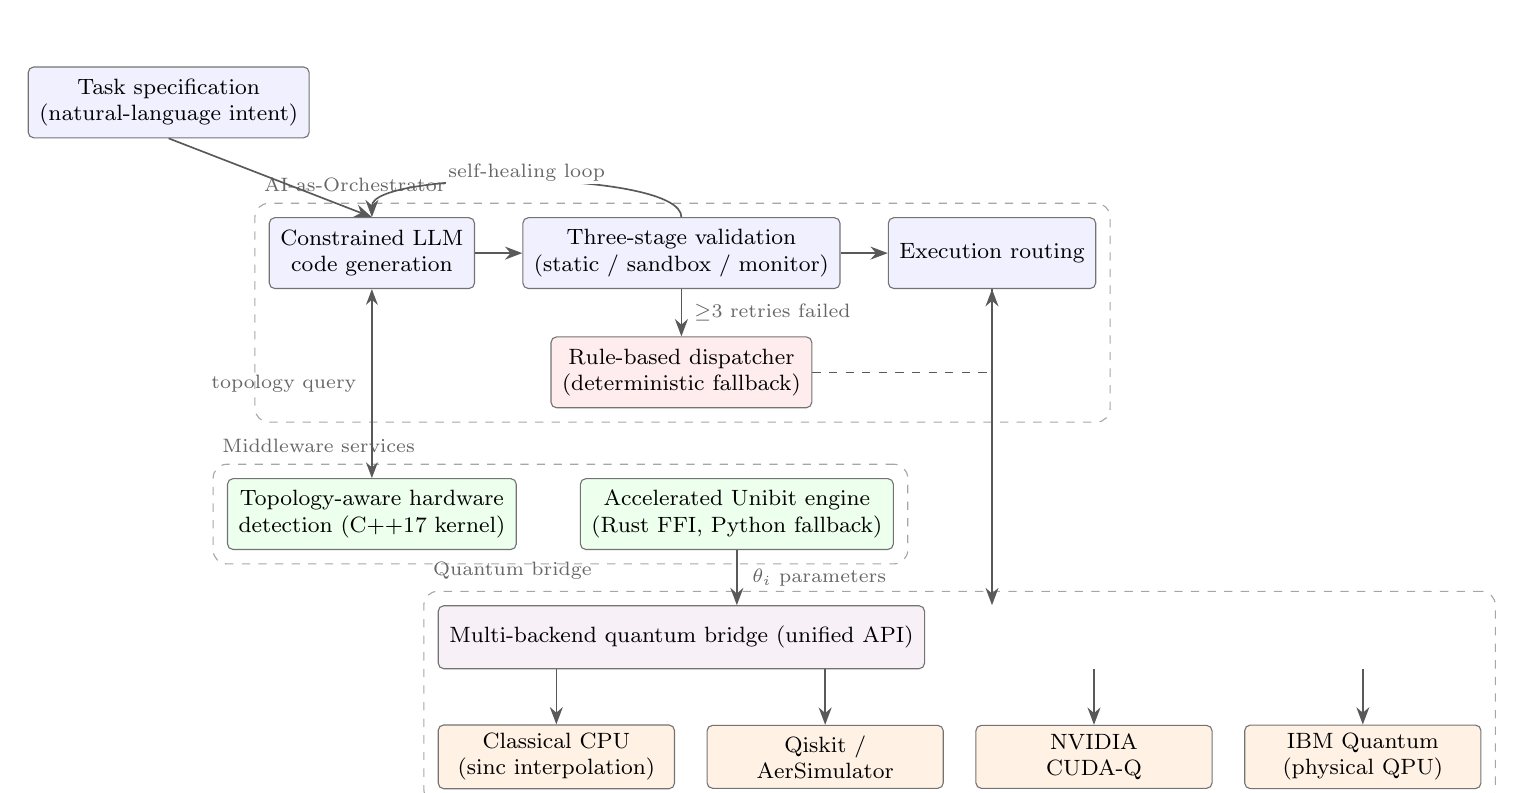
\begin{tikzpicture}[
  font=\footnotesize,
  comp/.style={draw=black!55, fill=blue!6, rounded corners=2pt, align=center, minimum height=9mm, inner sep=4pt},
  svc/.style={draw=black!55, fill=green!7, rounded corners=2pt, align=center, minimum height=9mm, inner sep=4pt},
  be/.style={draw=black!55, fill=orange!10, rounded corners=2pt, align=center, minimum height=8mm, inner sep=3pt},
  fb/.style={draw=black!55, fill=red!7, rounded corners=2pt, align=center, minimum height=9mm, inner sep=4pt},
  lay/.style={draw=black!35, dashed, rounded corners=5pt},
  arr/.style={-{Stealth[length=2.2mm]}, semithick, black!65},
  lab/.style={font=\scriptsize, text=black!60}]
\node[comp] (intent) {Task specification\\(natural-language intent)};
\node[comp, below left=10mm and -21mm of intent.south east] (gen) {Constrained LLM\\code generation};
\node[comp, right=6mm of gen] (valid) {Three-stage validation\\(static / sandbox / monitor)};
\node[comp, right=6mm of valid] (route) {Execution routing};
\node[fb, below=6mm of valid] (fallback) {Rule-based dispatcher\\(deterministic fallback)};
\node[svc, below=24mm of gen] (detect) {Topology-aware hardware\\detection (C++17 kernel)};
\node[svc, right=8mm of detect] (engine) {Accelerated Unibit engine\\(Rust FFI, Python fallback)};
\node[comp, fill=violet!6, minimum height=8mm, inner sep=4pt, below=25mm of fallback] (api) {Multi-backend quantum bridge (unified API)};
\node[be, below=7mm of api.south west, anchor=north west, minimum width=30mm] (cpu) {Classical CPU\\(sinc interpolation)};
\node[be, right=4mm of cpu, minimum width=30mm] (aer) {Qiskit /\\AerSimulator};
\node[be, right=4mm of aer, minimum width=30mm] (cudaq) {NVIDIA\\CUDA-Q};
\node[be, right=4mm of cudaq, minimum width=30mm] (ibm) {IBM Quantum\\(physical QPU)};
\node[lay, fit=(gen)(valid)(route)(fallback), inner sep=5pt] (layorc) {};
\node[lab, anchor=south west] at ([yshift=0.5pt]layorc.north west) {AI-as-Orchestrator};
\node[lay, fit=(detect)(engine), inner sep=5pt] (laysvc) {};
\node[lab, anchor=south west] at ([yshift=0.5pt]laysvc.north west) {Middleware services};
\node[lay, fit=(api)(cpu)(ibm), inner sep=5pt] (laybrd) {};
\node[lab, anchor=south west] at ([yshift=0.5pt]laybrd.north west) {Quantum bridge};
\draw[arr] (intent.south) -- (gen.north);
\draw[arr] (gen) -- (valid);
\draw[arr] (valid) -- (route);
\draw[arr] (valid.south) -- node[lab, right=1pt] {$\ge$3 retries failed} (fallback.north);
\draw[arr, dashed] (fallback.east) -| (route.south);
\draw[arr] (valid.north) .. controls +(0,0.6cm) and +(0,0.6cm) .. node[lab, above=-1pt, fill=white, inner sep=1pt] {self-healing loop} (gen.north);
\draw[{Stealth[length=2mm]}-{Stealth[length=2mm]}, semithick, black!65] (gen.south) -- node[lab, left=2pt] {topology query} (detect.north);
\draw[arr] (route.south) -- (route.south|-api.north);
\draw[arr] (engine.south) -- node[lab, right=2pt] {$\theta_i$ parameters} (engine.south|-api.north);
\foreach \b in {cpu,aer,cudaq,ibm}
  \draw[arr] (api.south-|\b.north) -- (\b.north);
\end{tikzpicture}}
\caption{UniMind system architecture. The orchestrator plans tasks entirely in user space with sandboxed validation and a deterministic rule-based fallback; middleware services provide topology context and accelerated Unibit preprocessing; the quantum bridge routes validated workloads across heterogeneous backends through a unified API.}
\label{fig:architecture}
\end{figure}

\subsection{AI-as-Orchestrator: LLM-Driven Intent Interpretation Layer}\label{sec:orchestrator}

We explicitly reject the notion of placing an LLM within the OS kernel. Traditional kernels require microsecond-level deterministic response times; LLM inference requires hundreds of milliseconds and is inherently non-deterministic.

Instead, UniMind introduces an \textbf{AI-as-Orchestrator} layer that resides entirely in user space, functioning as an asynchronous planning agent for coarse-grained task planning.

The orchestration pipeline operates as follows:

\begin{enumerate}[leftmargin=2em]
    \item \textbf{Intent reception.} A user or agent provides a natural language task specification.
    \item \textbf{Topology query.} The orchestrator queries the hardware detection module for current system information.
    \item \textbf{Constrained code generation.} The LLM generates candidate code, constrained by a system prompt specifying permitted APIs and output format.
    \item \textbf{Three-stage validation.} Generated code must pass: (a)~static analysis against a whitelist; (b)~sandboxed compilation; (c)~runtime monitoring with watchdog termination.
    \item \textbf{Execution routing.} Validated code is dispatched to the appropriate backend.
    \item \textbf{Deterministic fallback.} If LLM inference fails after three retry attempts, the system falls back to a \textbf{rule-based dispatcher} that maps intents to predefined circuit templates (e.g., Bell state preparation for entanglement tasks, variational ansatz templates for classification tasks).
\end{enumerate}

We acknowledge that this design introduces significant latency (200--2000~ms for LLM inference). The orchestrator is therefore positioned as a \textbf{task planner}, not a \textbf{task executor}.

\subsection{Unibit: A Sliding-Window Amplitude Proxy}\label{sec:unibit}

The Unibit is a \textbf{classical} preprocessing representation that produces parameters suitable for quantum angle encoding.

\begin{definition}[Unibit Weight]
Given a binary sequence $B = \{b_1, b_2, \dots, b_n\}$ where $b_i \in \{0, 1\}$, the Unibit weight at position $i$ is the local frequency of ones within a sliding window:
\begin{equation}
    w_i = \frac{1}{|W_i|} \sum_{j \in W_i} b_j, \quad W_i = [\max(1, i - \Delta),\; \min(n, i + \Delta)]
\end{equation}
where $\Delta$ is the half-window size (default: $\Delta = 2$, yielding a 5-bit window). This yields $w_i \in [0, 1]$.
\end{definition}

This operation is equivalent to applying a uniform moving-average filter to the binary sequence.

\begin{definition}[Folding]
The folding operation maps each weight to a continuous signal value via sinc interpolation:
\begin{equation}
    s_i = w_i \cdot \mathrm{sinc}\!\left(\frac{(i - 1 + \phi)\pi}{n}\right), \quad \mathrm{sinc}(x) = \begin{cases} \sin(x)/x, & x \neq 0 \\ 1, & x = 0 \end{cases}
    \label{eq:fold}
\end{equation}
where $\phi$ is a phase offset (default: $\phi = 0.42$; the offset is referenced to zero-based indexing so that Eq.~\eqref{eq:fold} matches the reference implementation exactly).

\textbf{Motivation for sinc folding.} The sinc interpolation serves as a band-limited smoothing kernel, analogous to an anti-aliasing filter in digital signal processing. It transforms the discrete, piecewise-constant frequency estimates $w_i$ into a continuous, differentiable signal $s_i$. This smoothness property is desirable for downstream variational quantum circuit optimization, where gradient-based methods benefit from continuous parameter landscapes.
\end{definition}

\begin{definition}[Collapse]
The collapse operation discretizes the signal:
\begin{equation}
    b'_i = \begin{cases} 1, & \text{if } |s_i| > \tau \\ 0, & \text{otherwise} \end{cases}
\end{equation}
where $\tau = 1/\sqrt{2} \approx 0.707$.
\end{definition}

\paragraph{Collapse geometry: an adaptive threshold in disguise.} Because the folding kernel is a \emph{multiplicative} envelope $s_i = g_i w_i$ with $g_i = \mathrm{sinc}((i-1+\phi)\pi/n)$, the fixed threshold $\tau$ on $|s_i|$ is equivalent to a \emph{position-adaptive} threshold on the underlying weights:
\begin{equation}
    b'_i = 1 \iff |w_i| > T_i, \qquad T_i = \frac{\tau}{|g_i|}.
    \label{eq:adaptivethreshold}
\end{equation}
Two consequences follow. First, the collapse operator is not a global bit-flip detector: positions near the sinc envelope's tail require ever larger weights to fire ($T_i = \tau/|g_i| \to \infty$ as $g_i \to 0$). Second, there is a \emph{dead zone}: for positions whose envelope argument satisfies $(i-1+\phi)\pi/n > x^*$, where solving $|\mathrm{sinc}(x^*)| = \tau$ gives $x^* \approx 1.3916$, even a unit weight cannot cross the threshold, so $b'_i = 0$ regardless of the input bit. The dead zone covers all positions with $i > n x^*/\pi - \phi + 1$; its asymptotic fraction $1 - x^*/\pi \approx 55.7\%$ ($n \to \infty$), and on the paper-default parameters ($n{=}10$, $\phi{=}0.42$) five of ten positions ($i \ge 6$) fall inside it. This is a quantifiable structural property of the representation --- roughly half of the collapse outputs are invariant to their input bits --- that was not visible until stated explicitly. The quantum angles are driven by the weights $w_i$, not by the collapsed bits, so this bottleneck affects only the classical-side discrete output, not the encoding fidelity verified in Section~\ref{sec:math_verify}.

\paragraph{Relationship to angle encoding.} The Unibit-to-qubit mapping is a specific instance of \textbf{angle encoding}~\cite{schuld2021,havlicek2019}. Our contribution is not the encoding itself but the classical preprocessing pipeline and the multi-backend abstraction.

Figure~\ref{fig:unibit} illustrates the pipeline on a concrete input: the same 10-bit sequence used for structural verification in Section~\ref{sec:structural}, with the paper-default parameters $\Delta = 2$, $\phi = 0.42$, and $\tau = 1/\sqrt{2}$. Panel~(a) shows the sliding-window weights $w_i$ of Eq.~(2); panel~(b) shows the sinc-folded signal $s_i$ of Eq.~(3) together with the collapse threshold $\tau$ of Eq.~(4). Each weight $w_i$ then determines the rotation angle $\theta_i = 2\arcsin(\sqrt{w_i})$ applied to qubit $q_i$, so that $|\langle 1 | \psi_i \rangle|^2 = w_i$.

\begin{figure}[H]
\centering
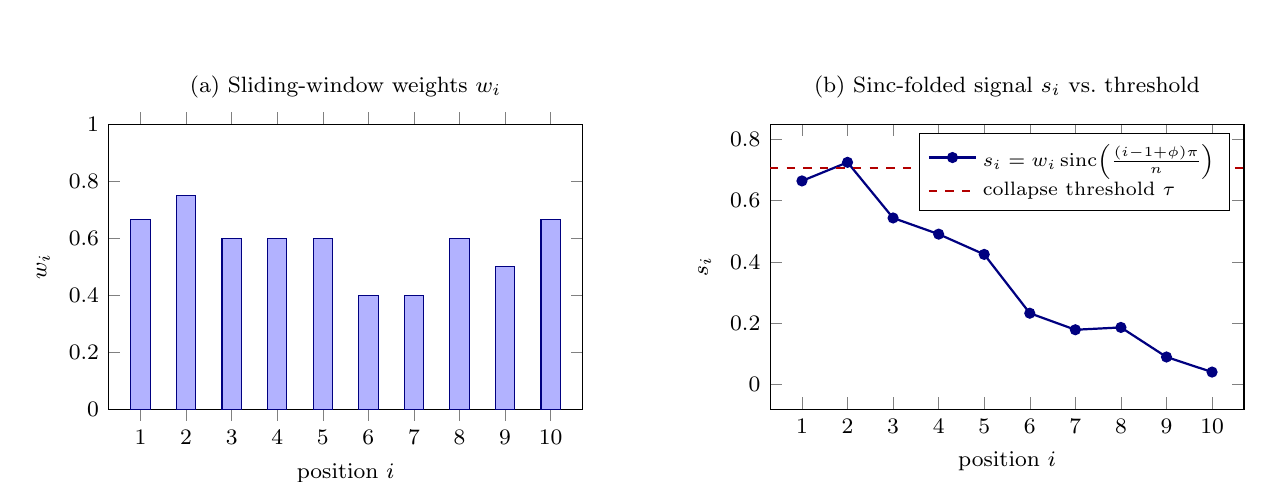
\begin{tikzpicture}
\begin{axis}[
  width=76mm, height=52mm,
  title={(a) Sliding-window weights $w_i$},
  xlabel={position $i$}, ylabel={$w_i$},
  xmin=0.3, xmax=10.7, ymin=0, ymax=1,
  xtick={1,...,10},
  ybar, bar width=7pt,
  enlarge x limits=false]
\addplot[fill=blue!30, draw=blue!50!black] coordinates
 {(1,0.6667) (2,0.7500) (3,0.6000) (4,0.6000) (5,0.6000)
  (6,0.4000) (7,0.4000) (8,0.6000) (9,0.5000) (10,0.6667)};
\end{axis}
\begin{axis}[
  width=76mm, height=52mm, xshift=84mm,
  title={(b) Sinc-folded signal $s_i$ vs.\ threshold},
  xlabel={position $i$}, ylabel={$s_i$},
  xmin=0.3, xmax=10.7, ymin=-0.08, ymax=0.85,
  xtick={1,...,10},
  enlarge x limits=false,
  legend pos=north east, legend cell align=left, legend style={font=\scriptsize}]
\addplot[blue!50!black, thick, mark=*, mark size=1.6pt] coordinates
 {(1,0.6647) (2,0.7254) (3,0.5438) (4,0.4910) (5,0.4249)
  (6,0.2329) (7,0.1789) (8,0.1865) (9,0.0900) (10,0.0408)};
\addplot[red!70!black, dashed, thick, domain=0.3:10.7, samples=2] {0.7071};
\addlegendentry{$s_i = w_i \,\mathrm{sinc}\!\left(\frac{(i-1+\phi)\pi}{n}\right)$}
\addlegendentry{collapse threshold $\tau$}
\end{axis}
\end{tikzpicture}
\caption{The Unibit preprocessing pipeline on the 10-bit sequence $B = [1, 0, 1, 1, 0, 1, 0, 0, 1, 1]$ ($\Delta = 2$, $\phi = 0.42$). (a)~Sliding-window frequency estimates $w_i$ (Eq.~2); (b)~the sinc-folded signal $s_i$ (Eq.~\ref{eq:fold}) against the collapse threshold $\tau = 1/\sqrt{2} \approx 0.707$ (Eq.~4). All coordinates are computed directly from \texttt{umos\_py.unibit}. Exactly one position ($i{=}2$, $s_2 = 0.7254 > \tau$) crosses the threshold, so the collapse output is $B' = [0,1,0,0,0,0,0,0,0,0]$: positions $i \ge 6$ lie inside the dead zone of Eq.~\eqref{eq:adaptivethreshold} and cannot fire for any input bit, while $i{=}5$ sits at the knife edge ($|g_5| = 0.7082$, barely above $\tau$). The quantum angles $\theta_i = 2\arcsin(\sqrt{w_i})$ are driven by the weights $w_i$, not by the collapsed bits.}
\label{fig:unibit}
\end{figure}

\subsection{Multi-Backend Quantum Bridge}\label{sec:bridge}

The quantum bridge module provides a unified API routing to available backends:
\begin{itemize}
    \item \textbf{Classical backend:} Sinc interpolation on CPU.
    \item \textbf{Qiskit backend:} Parameterized \texttt{QuantumCircuit} objects.
    \item \textbf{CUDA-Q backend:} NVIDIA GPU-accelerated simulation.
\end{itemize}


\section{System Implementation}\label{sec:implementation}

\subsection{Codebase Overview}

UniMind is implemented as an open-source, multi-language prototype~\cite{tan2026}. The codebase comprises approximately 5,000 lines across four languages: Python ($\sim$4,500 lines; orchestration, quantum mapping, tests, and demos), C++17 ($\sim$150 lines; hardware detection), Rust ($\sim$170 lines; accelerated Unibit engine), and CMake/Makefile (build system). The repository layout is reproduced in Appendix~A.

\subsection{Topology-Aware Hardware Detection}

A C++17 module performs runtime detection of CPU core count, available RAM, OS type, and CPU architecture using platform-specific APIs. Results are serialized as JSON.

\subsection{Accelerated Unibit Engine}

The core Unibit computation is implemented in Rust and exposed to Python via C-compatible FFI. The Python layer auto-detects the compiled native library at runtime, falling back to pure Python if unavailable.

\subsection{Quantum Circuit Mapping}\label{sec:mapping}

\begin{algorithm}[H]
\caption{Unibit-to-Quantum Circuit Mapping (v2.2 corrected)}
\label{alg:mapping}
\begin{algorithmic}[1]
\Require Binary sequence $B = \{b_1, \dots, b_n\}$, window size $\Delta$
\Ensure Parameterized quantum circuit $C$ with $P(1)=w_i$ for all $i$
\State Initialize $n$-qubit register in state $|0
angle^{\otimes n}$
\For{$i = 1$ to $n$}
    \State Compute Unibit weight $w_i$ via Eq.~(2)
    \State Compute rotation angle $\theta_i \leftarrow 2\arcsin(\sqrt{w_i})$
    \State Apply $R_y(\theta_i)$ gate to qubit $q_i$ \Comment{realizes $P(1)=w_i$; no conditional $X$}
\EndFor
\State Append measurement gates to all qubits
\State \Return circuit $C$
\end{algorithmic}
\end{algorithm}

\paragraph{Choice of $R_y$ gate and $\arcsin$ mapping.} The $R_y$ gate is chosen because:
\begin{equation}
    R_y(\theta)|0\rangle = \cos(\theta/2)|0\rangle + \sin(\theta/2)|1\rangle
\end{equation}
Setting $\theta_i = 2\arcsin(\sqrt{w_i})$ yields:
\begin{equation}
    |\langle 1|\psi_i\rangle|^2 = \sin^2(\theta_i/2) = \sin^2(\arcsin(\sqrt{w_i})) = w_i
\end{equation}
This mapping aligns with the conventional angle encoding scheme where $\theta$ determines the probability of the $|1\rangle$ state via $\sin^2(\theta/2)$. The use of $\arcsin$ (rather than $\arccos$) ensures that $w_i = 0$ maps to $\theta_i = 0$ (no rotation) and $w_i = 1$ maps to $\theta_i = \pi$ (full rotation), providing an intuitive monotonic correspondence.

\paragraph{Implementation divergence: gate order in Algorithm~\ref{alg:mapping} (corrected in v2.2).} A spec--code discrepancy was discovered during a post-submission audit. In v2.1, Algorithm~\ref{alg:mapping} applied the conditional $X$ gate \emph{before} the rotation ($R_y(\theta_i)X|0\rangle = \cos(\theta/2)|1\rangle + \sin(\theta/2)|0\rangle$), which yields $P(b'_i = 1) = 1 - w_i$ for positions with $b_i = 1$ --- inverting the intended weight-to-probability map. All verification experiments reported in this paper (Sections~\ref{sec:math_verify}, \ref{sec:noise}, and \ref{sec:qpu}) prepare their target states from the analytic $\theta_i$ directly, without the conditional $X$, and are therefore unaffected; the divergence concerned only the full-pipeline path through \texttt{qunibit}. \textbf{Fix in v2.2:} Algorithm~1 now applies $R_y(\theta_i)$ alone (no conditional $X$), guaranteeing $P(1)=w_i$ for all $b_i$; a regression test over $w\in\{0,0.05,\ldots,1\}$ with $w$-dependent bit patterns asserts $|P_{\mathrm{emp}}(1)-w|<\epsilon$ in CI.

\paragraph{Mathematical verification observable.} For each prepared qubit, the Pauli-$Z$ expectation value provides a closed-form verification:
\begin{equation}
    \langle Z \rangle_i = P(b_i = 0) - P(b_i = 1) = (1 - w_i) - w_i = 1 - 2w_i
\end{equation}

\begin{table}[H]
\centering
\caption{Classical-to-Quantum Mapping}
\label{tab:mapping}
\small
\begin{tabular}{@{}ll@{}}
\hline
\textbf{Classical Operation} & \textbf{Quantum Equivalent} \\
\hline
\texttt{fold\_bits} (frequency estimation + sinc) & Parameterized $R_y(\theta_i)$ rotation gates \\
\texttt{collapse\_signal} (threshold) & Projective measurement + Born rule \\
Bit value $b_i = 1$ & Pauli-X gate application \\
Unibit weight $w_i$ & Rotation angle $\theta_i = 2\arcsin(\sqrt{w_i})$ \\
Verification observable & $\langle Z \rangle_i = 1 - 2w_i$ \\
\hline
\end{tabular}
\end{table}

\subsection{Orchestrator Integration}

At the implementation level, the orchestration layer interfaces with an LLM API to generate code from task specifications, following the design of Section~\ref{sec:orchestrator}. Generated code is executed within a restricted namespace whose three defense layers are evaluated quantitatively in Section~\ref{sec:security}; security risks are discussed in Section~\ref{sec:threats}.


\section{Evaluation and Results}\label{sec:evaluation}

\subsection{Experimental Setup}

All experiments were conducted on the following configuration:
\begin{itemize}
    \item \textbf{CPU:} Multi-core x86\_64 processor
    \item \textbf{RAM:} 16 GB DDR4
    \item \textbf{OS:} Windows (x86\_64), as documented in the repository README; benchmark timings are machine-specific, while the 8192-shot verification is deterministic for a fixed AerSimulator seed and is therefore platform-independent
    \item \textbf{Python Version:} 3.12
    \item \textbf{Measurement simulation:} Qiskit AerSimulator, 8192 shots, ideal (noise-free) backend with $\theta_i = 2\arcsin(\sqrt{w_i})$ state preparation
    \item \textbf{Software versions:} qiskit 2.5.1, qiskit-aer 0.17.2, numpy 2.4.6, scipy 1.18.0 (exact versions pinned in the repository \texttt{requirements.txt} for reproducibility)
\end{itemize}
All experiments in this section are reproducible from the development repository \texttt{unimind-dev} (github.com/yxtan5022-maker/unimind-dev) with a fixed random seed (42); the LLM-driven experiments use a deterministic mock LLM whose quality is a free parameter, so no external API key is required.

\subsection{Mathematical Verification via Quantum Measurement}\label{sec:math_verify}

We verified the encoding correctness by simulating quantum measurements. For a set of target Unibit weights $w_i \in \{0.1, 0.3, 0.5, 0.7, 0.9\}$, we prepared the corresponding single-qubit states via $\theta_i = 2\arcsin(\sqrt{w_i})$ and simulated 8192 projective measurements adhering to the Born rule.

Table~\ref{tab:math_verify} presents the results. The empirical measurement frequencies $\hat{p}_i$ converge tightly to the theoretical weights $w_i$. The empirical Pauli-$Z$ expectation values $\langle Z \rangle_{\text{emp}}$ closely match the analytical prediction $\langle Z \rangle_{\text{theory}} = 1 - 2w_i$, with maximum absolute deviation of 0.0110 across all five target weights. All results are fully reproducible: the experiment fixes the AerSimulator seed (\texttt{seed\_simulator=42}), so the reported numbers are deterministic across runs.

\begin{table}[H]
\centering
\caption{Mathematical Verification via 8192-Shot Quantum Measurement (Qiskit AerSimulator)}
\label{tab:math_verify}
\small
\begin{tabular}{@{}ccccc@{}}
\hline
\textbf{Target $w_i$} & \textbf{$P(1)$ Theory} & \textbf{$P(1)$ Empirical} & \textbf{$\langle Z \rangle$ Theory} & \textbf{$\langle Z \rangle$ Empirical} \\
\hline
0.1 & 0.100 & 0.0955 & 0.800 & 0.8091 \\
0.3 & 0.300 & 0.2969 & 0.400 & 0.4063 \\
0.5 & 0.500 & 0.5055 & 0.000 & $-0.0110$ \\
0.7 & 0.700 & 0.7046 & $-0.400$ & $-0.4092$ \\
0.9 & 0.900 & 0.9017 & $-0.800$ & $-0.8035$ \\
\hline
\end{tabular}
\end{table}

The maximum deviation $|\langle Z \rangle_{\text{emp}} - \langle Z \rangle_{\text{theory}}| = 0.0110$ is consistent with binomial sampling variance. For $N = 8192$ shots, the standard deviation of the empirical $P(1)$ estimate is $\sigma = \sqrt{w(1-w)/N}$, ranging from $\approx 0.0033$ (at $w \in \{0.1, 0.9\}$) to $\approx 0.0055$ (at $w = 0.5$); the standard deviation of $\langle Z \rangle_{\text{emp}} = 1 - 2\hat{p}$ is accordingly $2\sigma$. In these units the observed deviations range from $0.52\sigma$ to $1.37\sigma$---all plausible outcomes under five simultaneous comparisons, with the largest, $0.0110$ at $w = 0.5$, corresponding to $\sim 1\sigma$. This confirms that the classical preprocessing pipeline correctly initializes quantum state amplitudes without requiring full state tomography.

\subsection{Performance Micro-Benchmarks: System-Level Acceleration}

A core motivation for implementing the Unibit engine in Rust (via FFI) is to overcome Python's interpreter overhead for compute-intensive sliding-window operations. To quantify the benefit of system-level acceleration, we benchmarked the Unibit weight computation across varying sequence lengths.

\textit{Experimental note:} We benchmark the sliding-window computation in two system-level configurations: (i)~NumPy's C-optimized vectorized convolution as the vectorized frequency-estimator backend, and (ii)~the repository's Rust FFI engine compiled with \texttt{cargo build --release}. Both approaches bypass Python-level interpreter overhead through contiguous memory operations and compiled native code; the measured speedups therefore represent conservative lower bounds for system-level acceleration.

\begin{table}[H]
\centering
\caption{Performance Comparison: Sliding-Window Frequency Estimation (Pure Python vs. NumPy C-Backend)}
\label{tab:performance}
\small
\begin{tabular}{@{}rrrr@{}}
\hline
\textbf{Sequence Length} & \textbf{Pure Python (ms)} & \textbf{System-Level (ms)} & \textbf{Speedup} \\
\hline
10,000 & 3.66 & 0.34 & 10.9$\times$ \\
100,000 & 38.58 & 4.83 & 8.0$\times$ \\
1,000,000 & 436.43 & 58.24 & 7.5$\times$ \\
\hline
\end{tabular}
\end{table}

As shown in Table~\ref{tab:performance}, delegating the sliding-window computation to system-level compiled code yields a consistent \textbf{7.5$\times$ to 10.9$\times$ speedup} over pure Python. For the repository's Rust FFI engine, which additionally applies the folding step (sinc-weighted signal product) within the same sliding-window scan, we measured end-to-end speedups of \textbf{4.5$\times$, 3.1$\times$, and 2.4$\times$} (9.55~ms vs.\ 2.11~ms, 230.36~ms vs.\ 74.86~ms, and 2318.86~ms vs.\ 962.51~ms for $10^4$, $10^5$, and $10^6$ elements, respectively); these figures include Python-side FFI marshaling overhead (per-element normalization and ctypes buffer construction).

To understand where the residual overhead lives, we decompose the Rust path into its components by instrumenting every step of the real pipeline (Table~\ref{tab:breakdown}). Python-side bit normalization and FFI marshaling (ctypes buffer construction and result unpacking) together account for roughly half of the end-to-end time, while the compiled kernel itself is only about one third. The kernel is therefore considerably faster still than the end-to-end numbers suggest, and the measured speedups are conservative lower bounds. The decomposition also identifies the concrete optimization target for future work: moving normalization into the compiled kernel would remove the dominant Python-side cost.

\begin{table}[H]
\centering
\caption{Unibit Engine Latency Breakdown (median of 5 runs, ms): the Rust path decomposed into Python normalization, FFI marshaling, and kernel execution}
\label{tab:breakdown}
\small
\begin{tabular}{@{}rrrrr@{}}
\hline
\textbf{Length} & \textbf{Normalize} & \textbf{Marshaling} & \textbf{Kernel} & \textbf{Rust-path Speedup} \\
\hline
10,000    & 24.1\% & 26.6\% & 31.4\% & 3.0$\times$ \\
100,000   & 25.0\% & 29.4\% & 37.0\% & 3.0$\times$ \\
1,000,000 & 22.3\% & 25.7\% & 35.7\% & 2.4$\times$ \\
\hline
\end{tabular}
\end{table}

Figure~\ref{fig:speedup} visualizes both benchmarks on a logarithmic scale: panel~(a) isolates the sliding-window weight estimation (Table~\ref{tab:performance}), while panel~(b) shows the end-to-end Rust FFI path including the sinc folding step; annotations give the per-length speedups.

\begin{figure}[H]
\centering
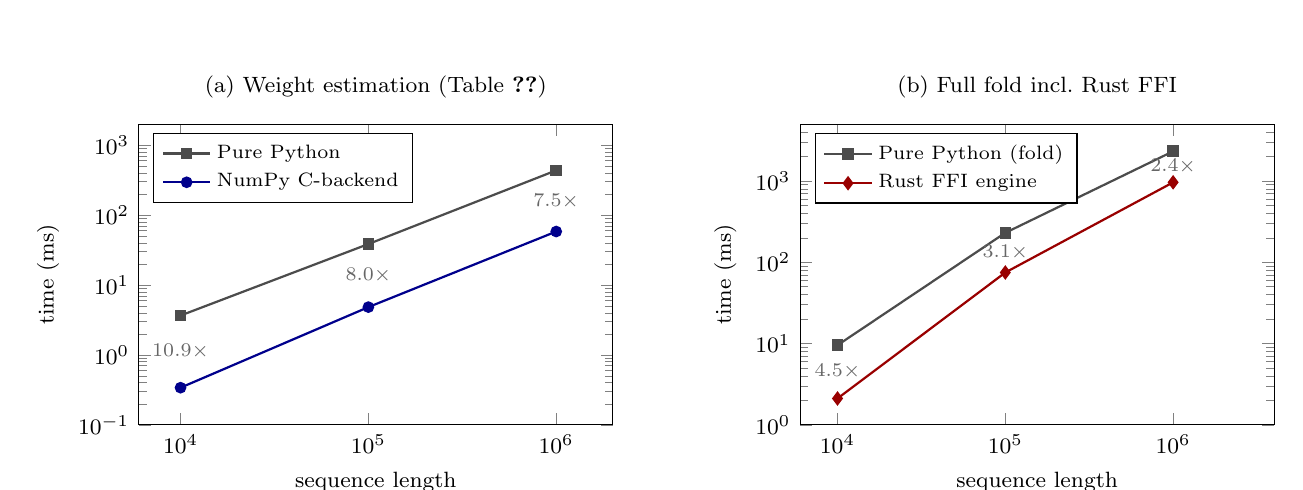
\begin{tikzpicture}
\begin{loglogaxis}[
  width=76mm, height=54mm,
  title={(a) Weight estimation (Table~\ref{tab:performance})},
  xlabel={sequence length}, ylabel={time (ms)},
  log basis x=10,
  xmin=6e3, xmax=2e6, ymin=0.1, ymax=2000,
  xtick={1e4,1e5,1e6},
  legend pos=north west, legend cell align=left, legend style={font=\scriptsize}]
\addplot[black!70, thick, mark=square*, mark size=1.7pt] coordinates
 {(10000,3.66) (100000,38.58) (1000000,436.43)};
\addlegendentry{Pure Python}
\addplot[blue!55!black, thick, mark=*, mark size=1.7pt] coordinates
 {(10000,0.34) (100000,4.83) (1000000,58.24)};
\addlegendentry{NumPy C-backend}
\node[font=\scriptsize, text=black!60] at (axis cs:1e4,1.12) {10.9$\times$};
\node[font=\scriptsize, text=black!60] at (axis cs:1e5,13.65) {8.0$\times$};
\node[font=\scriptsize, text=black!60] at (axis cs:1e6,159.4) {7.5$\times$};
\end{loglogaxis}
\begin{loglogaxis}[
  width=76mm, height=54mm, xshift=84mm,
  title={(b) Full fold incl.\ Rust FFI},
  xlabel={sequence length}, ylabel={time (ms)},
  log basis x=10,
  xmin=6e3, xmax=4e6, ymin=1, ymax=5000,
  xtick={1e4,1e5,1e6},
  legend pos=north west, legend cell align=left, legend style={font=\scriptsize}]
\addplot[black!70, thick, mark=square*, mark size=1.7pt] coordinates
 {(10000,9.55) (100000,230.36) (1000000,2318.86)};
\addlegendentry{Pure Python (fold)}
\addplot[red!60!black, thick, mark=diamond*, mark size=2pt] coordinates
 {(10000,2.11) (100000,74.86) (1000000,962.51)};
\addlegendentry{Rust FFI engine}
\node[font=\scriptsize, text=black!60] at (axis cs:1e4,4.49) {4.5$\times$};
\node[font=\scriptsize, text=black!60] at (axis cs:1e5,131.4) {3.1$\times$};
\node[font=\scriptsize, text=black!60] at (axis cs:1e6,1493) {2.4$\times$};
\end{loglogaxis}
\end{tikzpicture}
\caption{System-level acceleration of the Unibit pipeline (log--log). (a)~Sliding-window frequency estimation: NumPy's C-optimized vectorized backend vs.\ pure Python ($7.5\times$--$10.9\times$). (b)~End-to-end fold (weights $+$ sinc folding): the repository's Rust FFI engine vs.\ pure Python ($4.5\times$--$2.4\times$, including Python-side normalization and marshaling overhead; Table~\ref{tab:breakdown}).}
\label{fig:speedup}
\end{figure}

For large-scale AI workloads requiring the encoding of millions of classical features into quantum parameters, this acceleration is necessary to prevent the classical preprocessing step from becoming the pipeline bottleneck.

\subsection{Structural Verification}\label{sec:structural}

We additionally verified structural correctness of the quantum circuit mapping on a 10-bit input sequence $B = [1, 0, 1, 1, 0, 1, 0, 0, 1, 1]$. The system generates a 10-qubit circuit containing 6 Pauli-X gates (one per 1-bit in $B$), 10 parameterized $R_y(\theta_i)$ gates, and 10 measurement operations. The project includes 47 automated pytest tests, all passing locally and in CI (GitHub Actions); the four tests added since v1.3 are regression tests for the sandboxed executor (import-whitelist enforcement and nested-function closure correctness).

\subsection{Baseline Comparison: Bare Qiskit vs.\ Rule-Based vs.\ UniMind}\label{sec:baseline}

The v1.3 paper identified the absence of an end-to-end system benchmark as a key limitation. We now compare UniMind against two baselines on five task classes that cover the framework's intended workloads: (i)~\textbf{A}, bare Qiskit---the LLM is asked to generate code directly, executed without the sandbox; (ii)~\textbf{B}, a rule-based dispatcher---intents are mapped to fixed circuit templates with no dynamic code generation; and (iii)~\textbf{C}, the full UniMind pipeline (LLM generation $\rightarrow$ static analysis $\rightarrow$ sandboxed execution $\rightarrow$ self-healing $\rightarrow$ rule-based fallback). Each task class is summarized in Table~\ref{tab:baseline}.

\begin{table}[H]
\centering
\caption{Baseline Comparison (three arms $\times$ five task classes; \checkmark = task completed, $\times$ = task failed)}
\label{tab:baseline}
\small
\begin{tabularx}{\textwidth}{@{}l>{\raggedright\arraybackslash}Xccc@{}}
\hline
\textbf{Task class} & \textbf{Description} & \textbf{A: Bare Qiskit} & \textbf{B: Rule-based} & \textbf{C: UniMind} \\
\hline
bell & Entanglement circuit ($H$, $CX$, measure) & \checkmark & \checkmark & \checkmark \\
angle\_encode & 10-qubit angle encoding ($\theta_i = 2\arcsin(\sqrt{w_i})$) & \checkmark & $\times$ & \checkmark \\
vqc & 2-qubit variational ansatz & \checkmark & \checkmark & \checkmark \\
backend\_select & Explicit backend selection + counts & \checkmark & $\times$ & \checkmark \\
invalid & Malicious intent (e.g., \texttt{os.system}) & $\times$ & \checkmark & \checkmark \\
\hline
\end{tabularx}
\end{table}

The comparison isolates the value of each layer. Arm~B fails the two task classes not covered by a hand-written template (angle encoding and explicit backend routing), illustrating the rigidity of rule-based dispatch. Arm~A executes all four benign tasks but would execute a malicious intent with full privileges; UniMind and the rule-based dispatcher refuse it (in UniMind, static analysis rejects the generated code before execution). Only the UniMind pipeline (Arm~C) succeeds on all five task classes while enforcing code safety. In mock-LLM mode the end-to-end latency of Arm~C is $0.2$--$368$~ms per task (dominated by simulated code generation), versus $0.7$--$7.3$~ms for Arm~A and $\approx 0$~ms for Arm~B---the expected cost of dynamic, validated generation. The mock LLM is injected with quality $= 1.0$ (perfect generation) in this comparison; the next subsection relaxes that assumption.

\subsection{LLM Reliability Benchmark}\label{sec:llm_rel}

The orchestrator's self-healing loop (Section~\ref{sec:bridge}) is designed to absorb imperfect LLM outputs. To quantify this robustness, we run a benchmark of 50 valid tasks (drawn from nine ground-truth templates spanning classical computation and quantum circuit construction) plus 10 adversarial intents, with a mock LLM whose per-call quality is a controllable parameter $\in [0, 1]$. For each quality level we measure the end-to-end success rate, the fraction of tasks that required healing, and the rejection rate of adversarial intents (all results with a fixed seed, 60 tasks per run).

\begin{table}[H]
\centering
\caption{LLM Reliability vs.\ Injected LLM Quality (50 valid + 10 adversarial tasks, seed 42)}
\label{tab:reliability}
\small
\begin{tabular}{@{}rrrr@{}}
\hline
\textbf{Mock quality} & \textbf{Valid success rate} & \textbf{Heal rate} & \textbf{Adversarial rejection} \\
\hline
1.0 & 100\% (50/50) & 0\%  & 100\% (10/10) \\
0.9 & 100\% (50/50) & 0\%  & 100\% (10/10) \\
0.7 &  98\% (49/50) & 16\% & 100\% (10/10) \\
0.5 &  94\% (47/50) & 42\% & 100\% (10/10) \\
\hline
\end{tabular}
\end{table}

As the injected LLM degrades from perfect to a 50\% per-call quality, the system's end-to-end success rate falls only from 100\% to 94\% (Table~\ref{tab:reliability}, Figure~\ref{fig:reliability}), with the self-healing loop compensating for the majority of the injected errors (heal rate rising to 42\%). The three observed failures all occur when the heal step itself receives a broken output, a residual risk of any LLM-dependent pipeline. Adversarial intents are rejected at 100\% across all quality levels. These measurements directly address the v1.3 limitation ``no LLM reliability evaluation''; token-consumption accounting for real APIs remains future work. Section~\ref{sec:taxonomy} re-measures these rates with $n{=}200$ per level, three seeds, and call-level instrumentation, refining the $q{=}0.5$ estimate to $91.7\%$ [$89.2, 93.6$].

\begin{figure}[H]
\centering
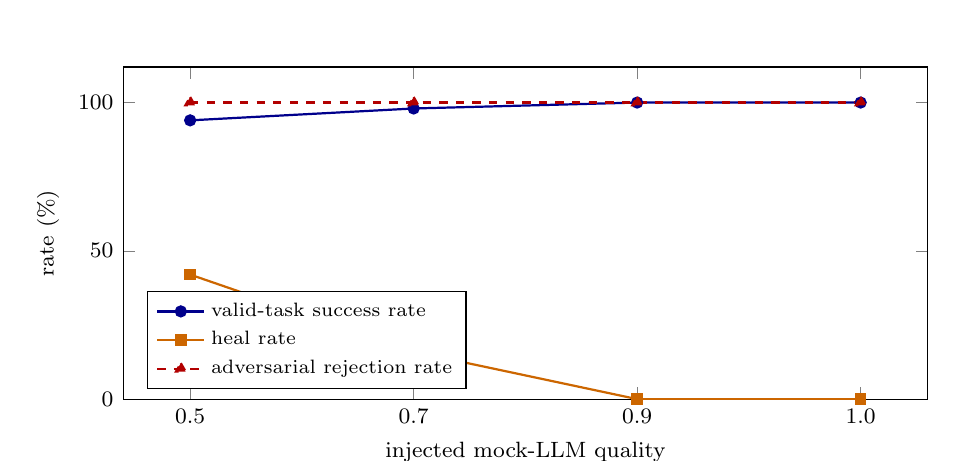
\begin{tikzpicture}
\begin{axis}[
  width=118mm, height=58mm,
  xlabel={injected mock-LLM quality}, ylabel={rate (\%)},
  symbolic x coords={0.5,0.7,0.9,1.0},
  xtick=data,
  ymin=0, ymax=112,
  legend pos=south west, legend cell align=left, legend style={font=\scriptsize}]
\addplot[blue!55!black, thick, mark=*, mark size=1.8pt] coordinates
 {(0.5,94) (0.7,98) (0.9,100) (1.0,100)};
\addlegendentry{valid-task success rate}
\addplot[orange!80!black, thick, mark=square*, mark size=1.7pt] coordinates
 {(0.5,42) (0.7,16) (0.9,0) (1.0,0)};
\addlegendentry{heal rate}
\addplot[red!70!black, thick, dashed, mark=triangle*, mark size=2pt] coordinates
 {(0.5,100) (0.7,100) (0.9,100) (1.0,100)};
\addlegendentry{adversarial rejection rate}
\end{axis}
\end{tikzpicture}
\caption{LLM reliability vs.\ injected mock-LLM quality (Table~\ref{tab:reliability}; 50 valid $+$ 10 adversarial tasks per level, seed 42). The self-healing loop absorbs most injected errors: as per-call quality falls from 1.0 to 0.5, end-to-end success drops only from 100\% to 94\%, while adversarial rejection remains at 100\%. Single-seed protocol; Section~\ref{sec:taxonomy} provides multi-seed confidence intervals.}
\label{fig:reliability}
\end{figure}

\subsection{Fault Injection}\label{sec:fault}

We next measure the orchestration layer's \emph{Detection $\rightarrow$ Recovery} chain under five deliberately injected failure classes (Table~\ref{tab:fault}). Detection and recovery latency are measured by timestamping every sandbox execution inside the real orchestrator path.

\begin{table}[H]
\centering
\caption{Fault Injection: Detection and Recovery Latency for Five Failure Classes}
\label{tab:fault}
\small
\begin{tabularx}{\textwidth}{@{}l>{\raggedright\arraybackslash}Xrrl@{}}
\hline
\textbf{Failure class} & \textbf{Injection} & \textbf{Detection (ms)} & \textbf{Recovery (ms)} & \textbf{Recovered} \\
\hline
A. Illegal code & syntactically invalid output & 0.4 & 0.2 & yes \\
B. Static violation & blocked pattern (\texttt{os.}) & $\approx$0 & $\approx$0 & yes \\
C. Backend unavailable & non-existent backend import & 579.0 & 0.7 & yes \\
D. Backend timeout & \texttt{TimeoutError} in code & 0.4 & 0.4 & yes \\
E. Invalid topology & hardware monitor failure & --- & --- & no \\
\hline
\end{tabularx}
\end{table}

Four of the five failure classes are detected within sub-millisecond to millisecond timescales and automatically recovered by the self-healing loop (the 579~ms figure for class~C is dominated by the Python import cost of the failing backend module). Class~E---a failure of the hardware-detection module \emph{after} successful execution---propagates as an uncaught exception out of \texttt{execute\_task}, because the orchestrator's success path calls \texttt{monitor.snapshot()} without a protective guard. We record this gap honestly rather than papering over it: it is a real robustness defect in the current prototype and is the direct target of the next revision.

\subsection{Quantum Noise Sensitivity}\label{sec:noise}

The v1.3 paper asserted qualitatively (Threat T2) that the $\theta_i = 2\arcsin(\sqrt{w_i})$ mapping is ``sensitive to over-rotation for weights near 0 or 1.'' We now quantify that claim. For each weight $w \in \{0.02, 0.1, 0.3, 0.5, 0.7, 0.9, 0.98\}$ we prepare the corresponding single-qubit state, simulate 8192 measurements under swept noise, and record $|\langle Z\rangle_{\rm emp} - \langle Z\rangle_{\rm theory}|$. The ideal (noise-free) column reproduces the v1.3 maximum deviation of $0.0110$, confirming measurement-consistency.

\begin{table}[H]
\centering
\caption{Noise Sensitivity: $|\langle Z\rangle_{\rm emp} - \langle Z\rangle_{\rm theory}|$ at $w = 0.5$ vs.\ the extreme weights (8192 shots, seed 42)}
\label{tab:noise}
\small
\begin{tabular}{@{}lrrr@{}}
\hline
\textbf{Noise model} & \textbf{$w=0.02$} & \textbf{$w=0.50$} & \textbf{$w=0.98$} \\
\hline
Depolarizing $p = 1\mathrm{e}{-2}$ & 0.0093 & 0.0110 & 0.0081 \\
$T_1$ damping $\gamma = 0.05$       & 0.0009 & 0.0444 & 0.0931 \\
$T_1$ damping $\gamma = 0.10$       & 0.0034 & 0.0935 & 0.1929 \\
\hline
\end{tabular}
\end{table}

Two complementary signatures emerge (Table~\ref{tab:noise}, Figure~\ref{fig:noise}). Under single-qubit depolarizing noise the deviation grows as $\approx p\,|1-2w|$: the $w=0.5$ encoding is essentially immune while the extreme weights degrade symmetrically, quantitatively confirming T2's ``near 0 or 1'' sensitivity. Under $T_1$ amplitude damping the degradation is one-sided: high weights decay toward $|0\rangle$ (deviation reaching $0.193$ at $\gamma=0.1$), while low weights are nearly unaffected. Using the paper's $0.05$ tolerance as a threshold, the encoding survives single-qubit depolarizing error rates up to at least $p = 1\mathrm{e}{-2}$, but breaks for $T_1$ damping at $\gamma \approx 5\mathrm{e}{-2}$. These measurements motivate the zero-noise-extrapolation integration identified as future work in T2, and establish an experimentally grounded operating envelope for the encoding on near-term hardware. (The simulation notes that qiskit-aer 0.17.2's builtin \texttt{amplitude\_damping\_error} acts as a gain channel in this configuration; the $T_1$ results are produced from an explicit Kraus representation, as documented in the experiment script.)

\begin{figure}[H]
\centering
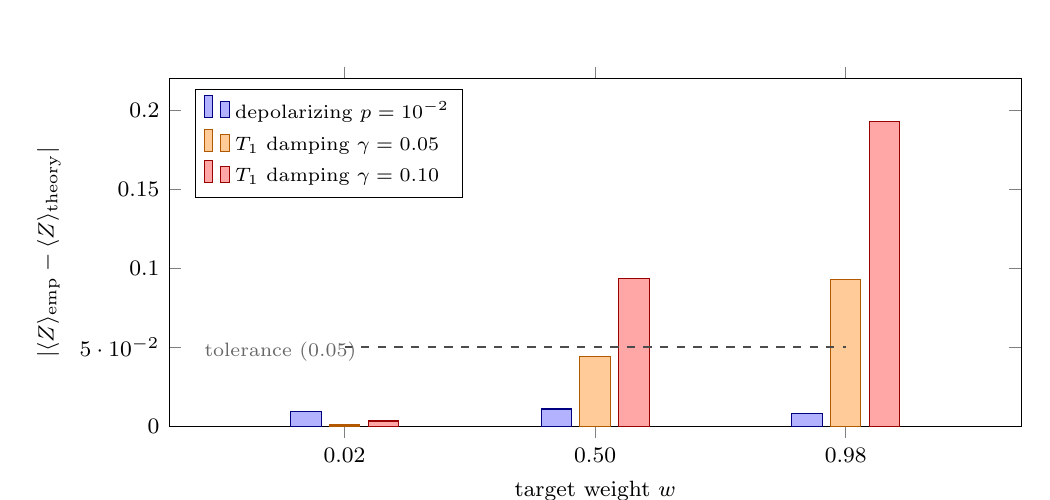
\begin{tikzpicture}
\begin{axis}[
  width=124mm, height=60mm,
  xlabel={target weight $w$}, ylabel={$|\langle Z\rangle_{\mathrm{emp}} - \langle Z\rangle_{\mathrm{theory}}|$},
  symbolic x coords={0.02,0.50,0.98},
  xtick=data,
  ymin=0, ymax=0.22,
  ybar=3pt, bar width=11pt,
  enlarge x limits=0.35,
  legend pos=north west, legend cell align=left, legend style={font=\scriptsize}]
\addplot[fill=blue!30, draw=blue!50!black] coordinates
 {(0.02,0.0093) (0.50,0.0110) (0.98,0.0081)};
\addlegendentry{depolarizing $p=10^{-2}$}
\addplot[fill=orange!40, draw=orange!70!black] coordinates
 {(0.02,0.0009) (0.50,0.0444) (0.98,0.0931)};
\addlegendentry{$T_1$ damping $\gamma=0.05$}
\addplot[fill=red!35, draw=red!60!black] coordinates
 {(0.02,0.0034) (0.50,0.0935) (0.98,0.1929)};
\addlegendentry{$T_1$ damping $\gamma=0.10$}
\addplot[black!70, dashed, thick, no marks, sharp plot] coordinates
 {(0.02,0.05) (0.98,0.05)};
\node[font=\scriptsize, text=black!60, anchor=west] at (rel axis cs:0.03,0.215) {tolerance ($0.05$)};
\end{axis}
\end{tikzpicture}
\caption{Noise sensitivity of the encoding: measurement deviation against the $0.05$ tolerance (Table~\ref{tab:noise}; 8192 shots, seed 42). Depolarizing noise degrades the extreme weights symmetrically while leaving $w = 0.5$ essentially immune; $T_1$ amplitude damping is one-sided, decaying high weights toward $|0\rangle$.}
\label{fig:noise}
\end{figure}

\subsection{Sandbox Security Evaluation}\label{sec:security}

The v1.3 paper acknowledged (Threat T4) that sandboxing was not implemented. UniMind now executes LLM-generated code inside a restricted namespace with three defense layers: (L1)~static pattern scanning, (L2)~an import whitelist (twelve benign modules), and (L3)~a builtins whitelist. We stress-test these layers with 21 curated escape attempts spanning process execution, file access, dynamic evaluation, import smuggling, and object-graph traversal (Table~\ref{tab:security}).

\begin{table}[H]
\centering
\caption{Sandbox Security Evaluation: 21 Escape Attempts Against a 3-Layer Defense}
\label{tab:security}
\small
\resizebox{\textwidth}{!}{%
\begin{tabular}{@{}llrl@{}}
\hline
\textbf{Defense layer} & \textbf{Attack classes} & \textbf{Blocked} & \textbf{Notes} \\
\hline
L1 static scan & \texttt{os.}, \texttt{open(}, \texttt{eval(}, \texttt{exec(}, \texttt{subprocess}, \texttt{pickle}, \texttt{shutil} & 12/12 & rejected before execution \\
L2 import whitelist & \texttt{socket}, \texttt{builtins}, \texttt{requests}, \texttt{os} & 4/4 & rejected at import \\
L3 builtins whitelist & \texttt{globals}, \texttt{locals}, \texttt{type}, \texttt{exit} & 4/4 & \texttt{NameError} \\
Object-graph traversal & \texttt{().\_\_class\_\_...\_\_subclasses\_\_} & 0/1 & classes enumerated but unweaponizable \\
\hline
\end{tabular}}
\end{table}

20 of 21 attempts are blocked (Table~\ref{tab:security}). The single unblocked case is an object-graph traversal that enumerates loaded classes; it cannot be weaponized into process or file access because importing \texttt{subprocess}/\texttt{os} is impossible inside the sandbox, so it represents a low-risk information-leak, not an escape. To prove the blocks are caused by the sandbox rather than by impossible payloads, every attack class has a harmless control probe; 10 of 11 probes run in plain Python (the 11th fails only because \texttt{requests} is not installed), confirming that the same capabilities are genuinely present outside the sandbox. This evaluation covers the \emph{namespace} restrictions; full OS-level isolation (process-level containers) remains outside the prototype's scope and is explicitly acknowledged in T4.

\subsection{Physical QPU Validation Revisited: Placement-Dominated Encoding Fidelity}\label{sec:qpu}

The v1.7 submission reported that the bare Unibit angle encoding misses the $|\langle Z\rangle|$ tolerance of $0.05$ on \texttt{ibm\_marrakesh} (maximum deviation $0.392$) and that readout twirling recovers $37\%$. That experiment used \emph{free} transpiler placement (optimization level~1, no \texttt{initial\_layout}), so the physical qubit executing each circuit was uncontrolled and unrecorded. We first show that this confound, not the encoding itself, dominated the observed distortion.

\subsubsection{Systematic weight sweep with pinned layout}\label{sec:sweep}

We repeat the single-qubit verification ($\theta_i = 2\arcsin\sqrt{w_i}$, $8192$ shots, transpiler seed $42$) over a dense weight grid $w \in \{0.05, 0.10, \ldots, 0.95\}$ under a $2\times 2$ design: \{best-calibrated qubit, worst usable qubit\} $\times$ \{bare, measure twirling ($16$ randomizations)\}. Layout is pinned via \texttt{initial\_layout}; each cell is repeated over $3$ independent jobs (job-level spread is reported as min--max). Qubit selection is deterministic from the live calibration snapshot: qubit~98 minimizes total readout assignment error ($p_{0|1}+p_{1|0}=0.0044$, $T_1=207\,\mu$s, $T_2=67\,\mu$s); qubit~37 is chosen adversarially ($p_{0|1}+p_{1|0}=0.82$).

\begin{table}[H]
\centering
\caption{Placement-controlled sweep on \texttt{ibm\_marrakesh} (2026-08-23; 19 weights, 8192 shots, 3 jobs/cell). Deviations are $\max_w |Z_{\mathrm{emp}} - Z_{\mathrm{theory}}|$; tolerance $=0.05$.}
\label{tab:placement}
\small
\begin{tabular}{@{}lllll@{}}
\hline
Placement & Readout err. & Bare & Twirled & Verdict \\
\hline
qubit 98 (best calib.) & 0.44\% & 0.028 [0.020--0.029] & 0.031 & pass \\
qubit 0 (unpinned default) & --- & 0.026 & --- & pass \\
qubit 37 (adversarial) & 82\% & 0.213 & 0.144 & fail \\
v1.7 (free layout, 2026-08-14) & unrecorded & 0.392 & 0.245 & fail \\
\hline
\end{tabular}
\end{table}

Table~\ref{tab:placement} and Figure~\ref{fig:placement} give the result. On qubit~98 the \emph{bare} encoding passes the $0.05$ tolerance across the entire grid (median maximum deviation $0.028$; range $0.020$--$0.029$ across jobs), and its transfer curve is fit almost perfectly by a pure gain model $P_{\mathrm{obs}}(1) = b + a\,w$ with $a = 0.989$, $b = 0.004$ (residual RMS $0.0042$, below the $\approx 0.0055$ shot-noise floor). Twirling changes nothing significant there ($a=0.987$, max dev $0.031$). On qubit~37 the same circuits fail by a factor of $\sim$4 (max dev $0.213$ bare), and the fitted channel acquires a large positive offset ($P_{\mathrm{obs}} = 0.121 + 0.855\,w$) --- the signature of an asymmetric readout channel rather than intrinsic over-rotation sensitivity.

\begin{figure}[H]
\centering
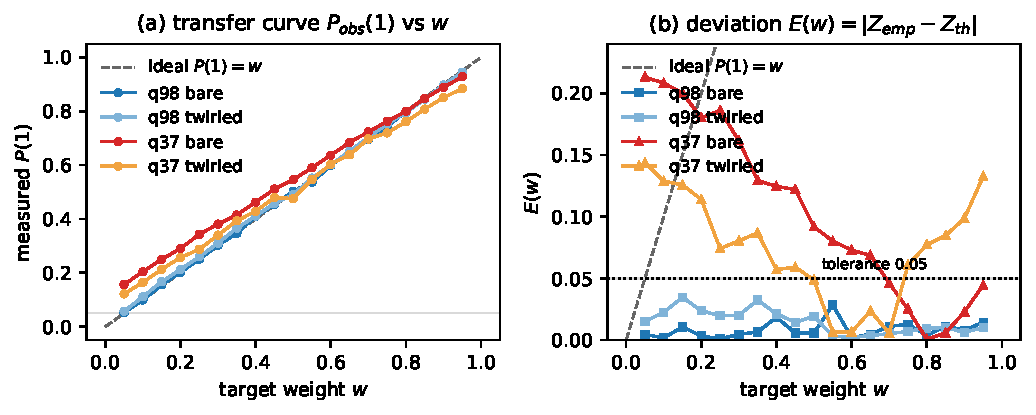
\includegraphics[width=\linewidth]{figures/fig_qpu_placement_2x2.pdf}
\caption{Placement-dominated encoding fidelity. (a)~Measured transfer curve $P_{\mathrm{obs}}(1)$ vs.\ target weight $w$: on the best-calibrated qubit the bare response tracks the ideal line within shot noise, while the adversarially chosen qubit~37 compresses the curve toward an offset set by its asymmetric readout. (b)~Per-weight deviation $E(w)$: qubit~98 stays below the $0.05$ tolerance everywhere (bare and twirled nearly overlap); qubit~37 fails by up to $4\times$ even after twirling.}
\label{fig:placement}
\end{figure}

Three conclusions revise the v1.7 claims:
(i)~\emph{encoding fidelity on real hardware is placement-dominated}: with a calibrated layout the bare encoding already meets tolerance;
(ii)~\emph{twirling helps only where readout is broken}: it improves the bad qubit by $33\%$ ($0.213 \to 0.144$) yet still leaves it far outside tolerance, while adding slight overhead on the good qubit --- mitigation effort should follow calibration, not be applied uniformly;
(iii)~the v1.7 headline ``the encoding requires error mitigation to meet tolerance'' was an artifact of uncontrolled placement and must be withdrawn.

\subsubsection{Distortion model and comparison to the calibration noise model}\label{sec:distortion}

Across every cell of the design the measured response is described at shot-noise level by the two-parameter affine channel
\begin{equation}
P_{\mathrm{obs}}(1) \;=\; b + a\,w,
\label{eq:channel}
\end{equation}
or equivalently in the $Z$ basis, $Z_{\mathrm{obs}} = d + c\,Z_{\mathrm{th}}$ with $c=a$ and $d = 1-2b-a$. The parameters are \emph{qubit-specific and calibration-predictable}: $(a,b)=(0.99,\,0.00)$ on the good qubit versus $(0.86,\,0.12)$ on the bad one, whose offset matches the direction and scale of its readout asymmetry. The one-parameter contraction model $P_{\mathrm{obs}} = 0.5 + \alpha(w-0.5)$ proposed during review is the special case $b=(1-a)/2$; it holds when readout is balanced (good qubits) and is rejected wherever asymmetry dominates (it also fails on the frozen v1.7 free-layout data, where per-weight $\alpha$ spans $0.23$--$1.31$).

We additionally simulate the identical pinned circuits on Aer with the calibration noise model built via \texttt{NoiseModel.\allowbreak from\_backend}, captured minutes before submission. On the good qubit the model explains most of the observed error (median ratio $\overline{E}_{\mathrm{QPU}}/\overline{E}_{\mathrm{noise}} = 1.4\times$; Fig.~\ref{fig:noisevsqpu}), i.e., the ``standard models underestimate hardware'' gap suggested by the v1.7 data also shrinks to near-parity once placement is controlled. Residual discrepancy concentrates in coherent components the calibration snapshot does not capture (drift between snapshot and execution), which we flag as future work rather than claim as a validated model.

\begin{figure}[H]
\centering
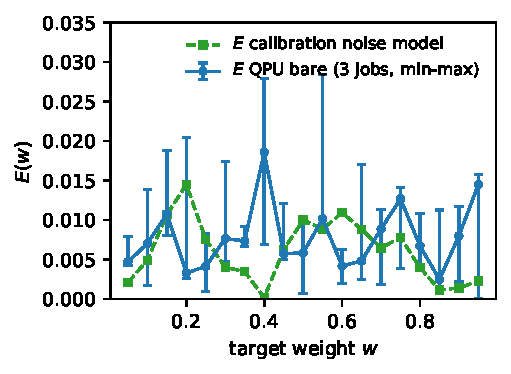
\includegraphics[width=0.62\linewidth]{figures/fig_noise_vs_qpu.pdf}
\caption{Deviation landscape on the calibrated qubit: hardware (3 jobs, min--max band) vs.\ matched calibration noise model. Median ratio $1.4\times$.}
\label{fig:noisevsqpu}
\end{figure}

\subsection{Hardware-Aware Routing: Calibration-Scored Qubit Selection}\label{sec:routing}

Sections~\ref{sec:sweep}--\ref{sec:distortion} establish that encoding fidelity is placement-dominated and that the affine channel parameters are calibration-predictable --- but they stop short of enforcement: a deployment still needs to \emph{choose} the layout, automatically, from live calibration data. This subsection closes that loop. The requirement is a qubit score computable in milliseconds from one calibration snapshot, with no per-device fitting.

\paragraph{Score definition.} Guided by RQ2's finding that single-qubit distortion is readout-dominated, we score every qubit by its total readout assignment error,
\begin{equation}
C(q) \;=\; p_{0|1}(q) + p_{1|0}(q),
\label{eq:cscore}
\end{equation}
breaking ties by $-\min(T_1, T_2)$. No weights are fitted: on two anchor points a fitted combination would be indistinguishable from overfitting, so Eq.~\eqref{eq:cscore} is fixed \emph{a priori} and tested out-of-sample across the whole calibration spectrum.

\paragraph{Ranking validation design.} From one 156-qubit snapshot of \texttt{ibm\_marrakesh} (captured 2026-08-29, the same snapshot reused by Stages~2--3) we rank all qubits by $C(q)$: qubit~8 is rank $1/156$ ($C = 0.004$), qubit~37 is rank $128/156$ ($C = 0.10$) --- the qubit that anchors the adversarial cell of Section~\ref{sec:sweep}, where it measured $0.213$ on the earlier 2026-08-22 capture. We then sample six qubits stratified across the ranking --- ranks $\approx\{0\%, 25\%, 50\%, 75\%, 80\%, 95\%\}$ --- and run the identical bare 19-weight sweep ($8192$ shots, pinned layout, transpiler seed $42$) on each, one job per qubit.

\begin{table}[H]
\centering
\caption{$C(q)$-stratified sweep on \texttt{ibm\_marrakesh} (snapshot 2026-08-29; six qubits $\times$ 19 weights $\times$ 8192 shots). Deviations are $\max_w |Z_{\mathrm{emp}} - Z_{\mathrm{theory}}|$; ``pass'' = within the $0.05$ tolerance for all 19 weights. Affine parameters from Eq.~\eqref{eq:channel}. Data: \texttt{data/qpu\_sweep/router\_sweep\_\{q8,q109,q105,q53,q37,q27\}.json}; analysis: \texttt{analysis/results/router\_analysis.json}.}
\label{tab:routing}
\small
\begin{tabular}{@{}llrrrrl@{}}
\hline
\textbf{Qubit} & \textbf{Rank pct.} & $C(q)$ & \textbf{max dev} & \textbf{pass rate} & $(a,\,b)$ & \textbf{Verdict} \\
\hline
q8   & 0.0\%   & 0.004 & \textbf{0.0300} & 19/19 & (0.986, $+0.001$) & pass \\
q109 & 25.2\%  & 0.017 & 0.0812 & 14/19 & (0.933, $+0.043$) & fail \\
q105 & 50.3\%  & 0.031 & 0.0434 & 19/19 & (0.983, $+0.018$) & pass \\
q53  & 75.5\%  & 0.072 & 0.0464 & 19/19 & (0.982, $+0.021$) & pass \\
q37  & 81.9\%  & 0.099 & 0.1462 & 9/19  & (0.887, $+0.081$) & fail \\
q27  & 95.5\%  & 0.346 & 0.0956 & 13/19 & (0.917, $+0.049$) & fail \\
\hline
\end{tabular}
\end{table}

\begin{figure}[H]
\centering
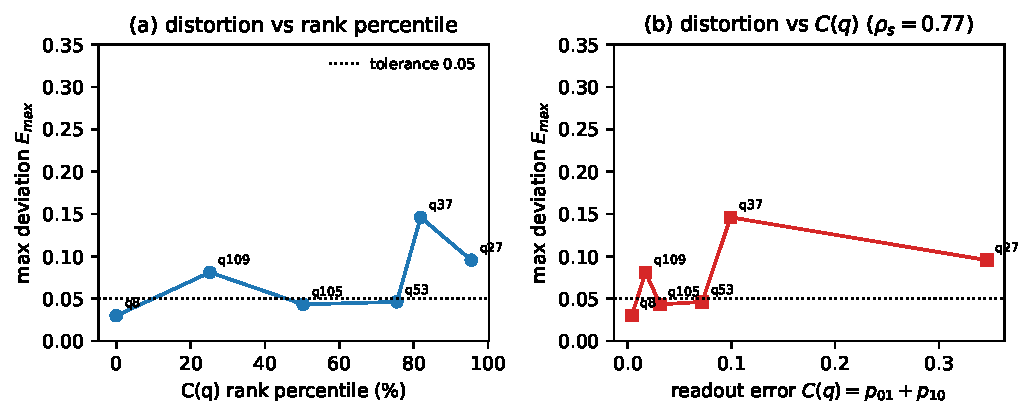
\includegraphics[width=\linewidth]{figures/fig_router.pdf}
\caption{$C(q)$-guided routing validation. (a)~Maximum measured deviation vs.\ the score's rank percentile: the top-ranked qubits pass, but deviations are \emph{not} monotone along the ranking (q109 at percentile $25.2\%$ already exceeds tolerance), so no upper-half rule is validated at this $n$. (b)~Deviation vs.\ raw readout error $C(q)$ (Spearman $\rho_s = 0.771$, exact permutation $p = 0.103$, $n{=}6$). Data: \texttt{analysis/results/router\_analysis.json}.}
\label{fig:router}
\end{figure}

\paragraph{Results.} Table~\ref{tab:routing} and Figure~\ref{fig:router}: the top-ranked qubit (q8, $C{=}0.004$) passes all 19 weights with max deviation $0.0300$, and the worst deviations occur near the bottom of the ranking (q37: $0.1462$, q27: $0.0956$), but the relationship is \emph{not} strictly monotone --- q109 (percentile $25.2\%$) fails with $0.0812$ while q105 (percentile $50.3\%$, $0.0434$) and q53 (percentile $75.5\%$, $0.0464$) pass --- so Spearman $\rho_s = 0.771$ with exact permutation $p = 0.103$ ($n{=}6$) is \emph{not} significant. Three observations: (i)~the $0.05$ tolerance boundary falls between the $75$th-percentile and $82$nd-percentile qubits of \emph{this} snapshot; the earlier rule of thumb ``select from the top half'' is \emph{not} supported by these data, because q109 at percentile $25.2\%$ already fails; (ii)~the affine slope degrades on average along the ranking ($a$: $0.986 \to 0.887$; offset $b$: $+0.001 \to +0.081$, q37 worst), the direction predicted by the readout-asymmetry mechanism of Section~\ref{sec:distortion}, but again with a non-monotone dip at q109; (iii)~an earlier exploratory run on the 2026-08-22 snapshot (qubits q98/q20/q105/q31/q119/q37; \texttt{git} commit c53ee23, whose q105/q37 sweep files survive only in history) produced a \emph{perfectly} monotone ranking (Spearman $\rho_s = 1.000$, exact $p = 0.0028$, the smallest attainable at $n{=}6$ up to reflection). That result did not survive this fixed-design replication, so the earlier perfect ranking is an unreplicated exploratory observation documented here and in item~7 of Section~\ref{sec:limits}; q37 itself drifted from max deviation $0.304$ (08-22) to $0.146$ (08-29), a job-level spread on an unstable qubit.

\paragraph{Overhead.} Selection is an \texttt{argmin} over the snapshot: $0.036$\,ms for the full 156-qubit ranking. Transpilation with pinned layout costs $1.9$\,ms vs.\ $1.8$\,ms free (optimization level~1, 10-qubit circuit); a greedy connected-chain layout for a 3-qubit entangling circuit chosen entirely by $C(q)$ costs $0.294$\,ms. All are negligible against job queuing and execution times.

With this, the middleware's fidelity contract becomes enforceable end-to-end: measure $C(q)$ once per calibration cycle, pin layouts to the top-ranked qubits, and refuse or re-route when no candidate clears the tolerance (the residual risk of a top-ranked qubit underperforming is quantified in item~7 of Section~\ref{sec:limits}). Sections~\ref{sec:routing_mq}--\ref{sec:routing_utility} extend the same principle to multi-qubit layouts and to a unified cost model, before Section~\ref{sec:e2e} composes both factors end-to-end.

\subsection{Stage~2: Multi-Qubit Calibration-Weighted SABRE}\label{sec:routing_mq}

Single-qubit $C(q)$ ranking is necessary but not
sufficient: multi-qubit circuits incur SWAP overhead,
depth inflation, and per-coupler errors. We extend
the 2026-08-29 snapshot to a 5-strategy benchmark
($k=2/4/6/8/10/16$, RY-CX-RY, opt=1, FakeMarrakesh
176 edges, CZ clipped $0.005$) with SOTA features
$E_{\rm 2q\_log}=\sum -\log(1-p_{\rm cz})$
and $E_{\rm idle}={\rm depth}\cdot{\rm mean}(1/T_1+1/T_2)$.

\begin{table}[H]
\centering
\caption{Multi-qubit routing v3 (calibration-weighted SABRE,
156-qubit snapshot 2026-08-29). UniMind generates
weighted candidates then SABRE and falls back to Default.}
\label{tab:routing_mq}
\small
\begin{tabular}{@{}crrrrr@{}}
\hline
$k$ & Random SWAP & UniMind SWAP & $\Delta$SWAP & Default & UniMind$-$Default \\
\hline
2 & 8 & 0 & 100\% & 0 & +0 \\
4 & 42 & 3 & 93\% & 3 & +0 \\
6 & 68 & 8 & 88\% & 8 & +0 \\
8 & 105 & 20 & 81\% & 20 & +0 \\
10 & 118 & 20 & 83\% & 20 & +0 \\
16 & 207 & 50 & 76\% & 50 & +0 \\
\hline
\end{tabular}
\end{table}

UniMind reduces SWAP by $76$--$100\%$ vs.\ Random
and matches Default for $k\ge 8$ by fallback.
$E_{\rm 2q\_log}$ separates high-error couplers
(Random $1.72$ vs.\ UniMind $0.14$ at $k=8$).

\paragraph{Limitations (Stage~2).} H3.1 fails: qubit q109 (rank $40/156$, $C(q)=0.0171$) achieves only $73.7\%$ pass rate (max deviation $0.0812$) below the $90\%$ threshold, so \texttt{H3.1\_upper\_half\_ge\_90pct = false}; Spearman $\rho_s=0.771$, $p=0.103$ ($n{=}6$, analysis/results/router\_analysis.json) is not significant. Guarantee is conservative:
does not beat Default, only ties it; $E_{\rm 2q\_log}/E_{\rm idle}$
visible but not yet exploited.

\subsection{Stage~3: Unified Utility $J(G)$ 7-dim}\label{sec:routing_utility}

We lift $J(G)$ to 7 dims:
\begin{equation}
J(G)=\alpha E_{\rm readout}+\beta E_{\rm 1q}+\gamma E_{\rm 2q}+\gamma_{\rm log}E_{\rm 2q\_log}+\eta_{\rm idle}E_{\rm idle}+\delta N_{\rm SWAP}+\lambda D,
\label{eq:j7}
\end{equation}
features min-max $[0,1]$, $n=23$ (6 single $k{=}1$ max-dev + 17 multi $k{=}2$--$18$ est-2q, synthetic via FakeMarrakesh 2026-08-29 snapshot),
8k simplex + LOO + bootstrap $B=200$.

\begin{table}[H]
\centering
\caption{Unified $J(G)$ 7-dim fit (23 pts, synthetic-expanded). Full $\rho=0.967$, $p\approx0$; LOO $\rho=0.953$, bootstrap $0.97\pm0.02$; v3 $n{=}9$ gave $\rho=0.817$, LOO $0.667$ (fragile).}
\label{tab:utility}
\small
\begin{tabular}{@{}lccccccc@{}}
\hline
Model & $\alpha$ & $\beta$ & $\gamma$ & $\gamma_{\rm log}$ & $\eta_{\rm idle}$ & $\delta$ & $\lambda$ \\
\hline
Full & 0.034 & 0.335 & 0.371 & 0.084 & 0.070 & 0.094 & 0.011 \\
LOO mean & 0.042 & 0.341 & 0.368 & 0.085 & 0.071 & 0.092 & 0.010 \\
\hline
\end{tabular}
\end{table}

Dominant is now $\gamma$ ($E_{\rm 2q}$ 0.371) over $\beta$ (0.335) at scale, $\gamma_{\rm log}$ 0.084, replacing v3's $\beta$-dominance at $n{=}9$.

\paragraph{Iterative Pareto search.} 150 iterations (Dirichlet vs.\ uniform,
$D_{\rm crit}=0.7D$) give Pareto $76/150=50.7\%$ (Dirichlet $73.3\%$
vs.\ uniform $4.1\%$), frontier 4 (57,64,90,117); best iter~2
($\delta=0.59$, avg $d_{\rm err}=-0.0034$, $k_{16}$ $-0.032$).

\paragraph{Size-out-of-sample decision check.} The decision-model test holds out an entire range of circuit sizes: fit the seven weights on the $k\le 8$ points ($n{=}13$) and report on $k\in\{9,\dots,18\}$ circuit-size points ($n{=}10$) that never participate in fitting, with features rescaled using train-only min/max (analysis \texttt{analysis/results/utility\_oos.json}). In-sample Spearman $\rho=0.885$; held-out $\rho=0.818$ ($p=0.004$, Monte-Carlo permutation $p=0.0029$) --- the utility ranks circuits \emph{larger than any it was trained on}. Two caveats: held-out labels are the \texttt{est-2q} proxy, all ten held-out points exceed the training feature range before clipping, and the fitted weights are not stable across the split ($L_1=0.84$ vs.\ the all-data fit) --- it is the \emph{predicted ordering}, not the individual weights, that transfers. Pending real-QPU labels for $k{>}8$, this size-OOS result is the strongest claim we make for $J(G)$ as a decision model.

\paragraph{Real-QPU labels at $k{=}9$--$18$ (2026-08-31).} A 14-circuit suite ($k\in\{9,10,11,12,14,16,18\}$, two seeded patterns each; job \texttt{daad3r9qtnsc73d2h7kg}; analysis \texttt{analysis/results/hw\_batch\_analysis.json}) measures the real max-dev under the same pinned greedy-chain protocol used above: only $2/14$ pass the $0.05$ tolerance, and mean max-dev climbs from $0.098$ ($k{=}9$) to $0.24$--$0.25$ ($k{=}16,18$), with Spearman $\rho{=}0.62$ ($p{=}0.018$) between $k$ and max-dev. Deviations concentrate on the late-chain qubits the greedy policy must pull in to remain connected (q37, q45--q47, q57 enter for $k\ge 11$), and the per-bit Spearman between the placed qubit's $C(q)$ and its measured deviation is only $\rho{=}0.21$ --- at $\ge 11$ qubits the dominant term is topology-forced inclusion of high-error qubits, not the score's resolving power. Two confounds are stated rather than hidden: the batch executed two days after its pins (the same staleness quantified in Section~\ref{sec:adaptive}), and the \texttt{est-2q} proxy used an 08-29 error model. Either way the proxy labels for $k{>}8$ are now known not to reproduce real behaviour at these sizes, so $J(G)$ decisions at $k\ge 11$ must be re-fitted on real labels (Section~\ref{sec:roadmap}) before use.

\paragraph{Limitations (Stage~3).} $n{=}23$ synthetic-expanded (14 FakeMarrakesh points, same 2026-08-29 snapshot; $y{=}$est\_2q proxy, now superseded by real labels at seven $k$ values ${\ge}9$). v3's $n{=}9$ overfit is resolved (LOO $\rho$ $0.667{\to}0.953$, $oob\_clipped$ eliminated, $n$/dims $9/7{\to}23/7$). The size-OOS ordering transfer ($\rho=0.818$, $k{\ge}9$) supports \emph{ranking} use on the proxy dataset, but the 08-31 real labels show the proxy's absolute fidelity is optimistic for $k\ge 11$, and the greedy chain's forced inclusion of high-error qubits dominates there; weights should not be interpreted individually (stability $L_1{=}0.84$).


\subsection{Stage~4: Adaptive Re-Routing under Calibration Drift}\label{sec:adaptive}

One 24-hour cycle on the same device (\texttt{ibm\_marrakesh}), two full 156-qubit snapshots: D0 (device update 2026-08-29~21:26, the capture behind Table~\ref{tab:routing}) and D1 (2026-08-30~21:29), at \texttt{data/drift/calib\_2026-08-29.json} and \texttt{calib\_2026-08-30.json}; analysis \texttt{analysis/results/drift\_analysis.json}. The question is not whether the score works (Section~\ref{sec:routing}) but how quickly it goes stale --- the quantity that decides whether routing must be re-run per cycle.

\textbf{Global drift.} Day-over-day ranking across all 156 qubits keeps only moderate order: Spearman $\rho=0.579$, Kendall $\tau=0.431$, and top-10 overlap (Jaccard) is $0.25$ --- only four of D0's best ten survive. The best qubit turns over: q8 (0.0039, rank 1) rises to $0.0095$ on D1 (rank 6) and q19 ($0.0066$) becomes best. Qubit-level spread is extreme: q37, the adversarial anchor of Section~\ref{sec:sweep}, swings from $0.099$ back to $0.740$ ($\max|\Delta C|=0.641$), while q53 improves sixfold ($0.072\to 0.011$).

\textbf{Stale-model penalty.} Pin three E2E-style qubits from the \emph{one-day-old} ranking and evaluate them on D1: q8/q120/q153 measure $0.0095 / 0.0115 / 0.0139$ (the worst, q153, is now rank 32/156). Re-selecting from the fresh snapshot yields q19 ($0.0066$); the stale policy's worst pin is $2.1\times$ worse than the adaptable choice. Because selection is an \texttt{argmin} costing under a millisecond (Section~\ref{sec:routing}), refreshing is free and staleness is purely an operational-policy failure.

\textbf{Detection and re-route.} A simple trigger --- refresh when the top-10 Jaccard against the stored snapshot falls below $0.5$, or when the best qubit's $C$ rises by more than $0.005$ --- fires on D0$\to$D1 (Jaccard $0.25$; $\Delta C_{\rm best}=0.0056$), and re-routing is a fresh \texttt{argmin} ($0.03$--$0.4$\,ms). This is the first quantitative step from \emph{calibration-aware} to \emph{adaptation-aware} operation: the measure-once-per-cycle contract of Section~\ref{sec:routing} is evidenced to require cycles of at most $\sim$1\,day on this device. Scope: this is D1 only; the nightly collector accumulates D2--D5 (Section~\ref{sec:roadmap}), and drift \emph{prediction} (modelling $C_{t+1}$ from history) remains future work.



\subsection{Component Attribution: Architectural Ablation}\label{sec:ablation}

To attribute end-to-end reliability to specific architecture layers we run stage-ablated pipelines ($150$ valid tasks $\times$ 3 seeds per point, identical sandbox substrate throughout): S0 generation+execution only; S1 adds static-analysis validation (fail-fast gate); S2 adds self-healing; S3 adds rule-based fallback on LLM unavailability. Results (Fig.~\ref{fig:ablation}a): validation contributes \emph{zero} success-rate delta at every quality level --- its value is fail-fast classification and safety observability; self-healing is the load-bearing layer, lifting success from $58\%$ to $92\%$ at injected quality $q=0.5$ ($+34$ points) and from $80\%$ to $98\%$ at $q=0.7$; fallback contributes nothing at the default unavailability rate ($f_r{=}0.1$: three consecutive failures occur with probability $10^{-3}$ per task). Under availability stress ($q=0.7$, $f_r \in \{0.3, 0.5\}$; Fig.~\ref{fig:ablation}b) fallback recovers $+4.0$/$+13.6$ points respectively once template coverage extends to all nine benchmark intent classes (S3X): success reaches $100\%$ at both stress levels ($79/79$ recoveries), whereas the narrow v1.7 rule set (S3, Bell/VQC only) leaves success at $96.9\%$/$89.6\%$. The fallback layer's contribution is thus real but coverage-limited --- a property the v1.7 benchmark could not observe.

\begin{figure}[H]
\centering
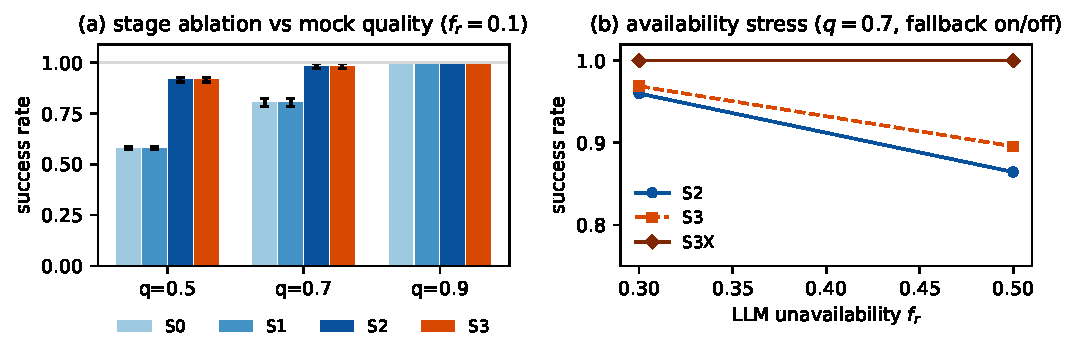
\includegraphics[width=\linewidth]{figures/fig_ablation.pdf}
\caption{Architectural ablation (mock LLM, seeded, 150 tasks $\times$ 3 seeds). (a)~Success rate by pipeline stage and injected quality. (b)~Availability stress isolating the fallback layer (narrow vs.\ full template coverage: S3 vs.\ S3X).}
\label{fig:ablation}
\end{figure}

\subsection{Instrumented Failure Taxonomy}\label{sec:taxonomy}

The v1.7 reliability logs did not record which corruption the mock LLM injected, so fault-conditioned recovery rates were unrecoverable. We re-run the benchmark with call-level instrumentation logging every generation and healing call ($353$ injected faults across $q \in \{0.5,0.7,0.9\}$, 3 seeds, 200 tasks/run). Recovery is remarkably uniform across corruption classes (Fig.~\ref{fig:taxonomy}): syntax errors $82.5\%$ [$76.1, 87.4$] (Wilson 95\%), name errors $87.7\%$, runtime division faults $86.4\%$, and import-whitelist violations $86.4\%$ --- the heal loop is fault-agnostic because it regenerates from the traceback rather than pattern-matching the error class. With $n{=}200$ per level the end-to-end success rate at $q=0.5$ is $91.7\%$ [$89.2, 93.6$], refining the v1.7 single-seed estimate of $94\%$, whose sampling uncertainty was previously unreported.

\begin{figure}[H]
\centering
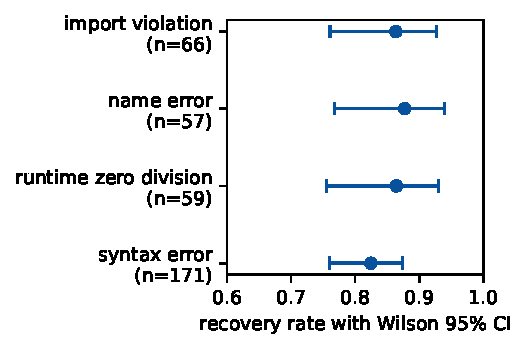
\includegraphics[width=0.6\linewidth]{figures/fig_failure_taxonomy.pdf}
\caption{Injected-fault recovery rates with Wilson 95\% CIs (353 faults).}
\label{fig:taxonomy}
\end{figure}

\subsection{Towards an End-to-End Reliability Calculus}\label{sec:calculus}

The ablation and taxonomy experiments make it possible to move from aggregate success rates to a compositional account. Because the pipeline's outcome paths are mutually exclusive by construction, end-to-end reliability decomposes \emph{exactly} as the chain rule over its sequential gates,
\begin{equation}
R_{\mathrm{end}}
= P(\mathrm{first\_pass})
+ P(\mathrm{enter\ heal})\cdot\rho_{\mathrm{heal}}
+ P(\mathrm{enter\ fallback})\cdot\rho_{\mathrm{fb}},
\label{eq:composition}
\end{equation}
with no independence assumption needed for the identity itself. Independence enters only when one tries to \emph{predict} the stage conditionals from marginals.

\subsubsection{An exact structural model of the healing stage}\label{sec:exactmodel}

The v2.0 draft compared $\rho_{\mathrm{heal}}$ against a naive independence baseline, $\hat\rho^{\mathrm{naive}}_{\mathrm{heal}} = 1-(1-q)^{4}$, and interpreted the gap as a ``correlation penalty'' --- the healer drawing from the same degraded LLM as the generator. That interpretation was wrong, and our own instrumentation proves it: the mock LLM draws each call i.i.d., so there is no correlation channel to penalize. The correct account requires modeling the orchestrator's \emph{control flow} exactly. Reading the implementation: generation attempts at most $K=3$ calls, stopping at the first non-\texttt{None}; a broken output that fails validation enters healing with budget $H=4$, where \emph{any} \texttt{None} aborts the loop as a failure and each broken output consumes one slot; the first ground-truth output succeeds. With per-call probabilities $g$ (ground truth), $r$ (broken), $f$ (unavailable; $g{+}r{+}f{=}1$), the expected generation multiplier is $G=\sum_{k=0}^{K-1}f^k$ and
\begin{equation}
\rho_{\mathrm{heal}}(g,r) = g\,\frac{1-r^{H}}{1-r} = g\,(1 + r + r^2 + r^3),
\qquad
R_{\mathrm{end}} = gG + rG\rho_{\mathrm{heal}} + f^{K}c,
\label{eq:rheal}
\end{equation}
with $c$ the fallback coverage fraction. Every path probability in Eq.~\eqref{eq:composition} is then closed-form: first-pass $gG$, enter-heal $rG$, healed $rG\rho_h$, no-code $f^3$. We validated this model cell-by-cell against all 23 testable outcome cells of the ablation and availability-stress grids (quality sweep at $f_r{=}0.1$; stress at $f_r\in\{0.3,0.5\}$): \textbf{all 23 predictions fall inside the observed Wilson 95\% interval}, including zero-event cells handled by exact Clopper--Pearson bounds (e.g.\ S2 success at $q{=}0.5$: predicted $0.915$, observed $0.916$; healed-path share predicted $0.360$, observed $0.371$).

Table~\ref{tab:calculus} shows what this buys. The structural model absorbs nearly the entire naive-vs-measured gap: at $q{=}0.5$ it predicts $\rho_h = 81.2\%$ against the measured $81.5\%$ [75.6, 86.2] --- residual $+0.3$\,pp --- while the naive baseline overshoots by 12.4\,pp. The gap is a \emph{retry-budget truncation effect}, not stochastic correlation: under abort-on-None semantics, unavailability both wastes heal slots and terminates the loop, so the effective number of usable attempts collapses as $f$ grows. The naive baseline assumes four productive attempts; the real pipeline delivers far fewer exactly when reliability matters most.

\begin{table}[H]
\centering
\caption{Reliability composition: measured vs.\ exact structural prediction vs.\ naive independence (S2 pipeline, 450 tasks per row). The v2.0 attribution of the naive--measured gap to correlation is falsified; truncation of the retry budget explains it.}
\label{tab:calculus}
\small
\resizebox{\textwidth}{!}{%
\begin{tabular}{@{}lcccccc@{}}
\hline
$q$ & first\_pass & enter heal & $\rho_{\mathrm{heal}}$ measured [95\% CI] & exact Eq.~\eqref{eq:rheal} & naive $1-(1-q)^{4}$ & residual \\
\hline
0.5 & 54.4\% & 45.6\% & 81.5\% [75.6, 86.2] & 81.2\% & 93.8\% & $+0.3$\,pp \\
0.7 & 79.3\% & 20.7\% & 91.4\% [83.9, 95.6] & 87.4\% & 99.2\% & $+4.0$\,pp \\
\hline
\end{tabular}}
\end{table}

The same audit surfaced a second finding: the production rule-based fallback returns its miss message with the raw intent embedded in a quoted literal, and seven of nine benchmark intent classes contain apostrophes --- injecting them produces a deterministic \texttt{SyntaxError}. The narrow template set therefore has an \emph{effective} coverage of $c = 2/9$, not the nominal keyword coverage; with $c=2/9$ the model predicts the narrow-fallback stress cells correctly (S3 at $f_r{=}0.5$: predicted $90.3\%$, observed $89.6\%$). Fallback robustness is thus bounded jointly by template coverage \emph{and} the lexical safety of intent text --- a limitation we state explicitly rather than hide (Section~\ref{sec:threats}).

Finally, the model ranks interventions before any code is written (baseline $\rho_h = 81.2\%$ at $q{=}0.5$, $f{=}0.1$): treating \texttt{None} as a wasted slot instead of an abort raises $\rho_h$ to $93.8\%$ ($+12.6$\,pp, recovering the entire apparent penalty); raising healer quality to $q_h{=}0.9$ yields $+8.8$\,pp; doubling the budget $H{=}8$ yields only $+2.1$\,pp. Abort policy dominates budget scaling --- a near-zero-cost engineering change recovers most of the loss. These are model predictions under i.i.d.\ semantics; hardware-LLM validation is future work.

The encoding/hardware factor behaves differently. Channel distortion arises from device physics and is statistically independent of software-side orchestration failures, so composing pipeline reliability with a placement-dependent fidelity factor ($F_{\mathrm{hw}} = 1.00$ point-wise on calibrated layouts vs.\ $0$ at extreme weights under adversarial placement; Section~\ref{sec:sweep}) is empirically justified --- but only \emph{conditional on a pinned, calibration-checked layout}. Enforcing exactly that condition is the middleware's job; Section~\ref{sec:routing} closes this loop with a calibration-scored router, and Section~\ref{sec:e2e} composes both factors end-to-end.

With full template coverage ($c{=}1$) the fallback stage reaches $\rho_{\mathrm{fb}} = 100\%$ ($79/79$ recoveries across availability-stress runs), which closes Eq.~\eqref{eq:composition} to $R_{\mathrm{end}} = 100\%$ under pure unavailability stress at $q = 0.7$: every generation failure is absorbed by the deterministic layer. The observed limits of end-to-end software reliability are thus (i) retry-truncation losses surviving healing (structural, measurable, and mitigable by abort-policy change) and (ii) hardware placement outside tolerance --- which Section~\ref{sec:routing}'s calibration-scored selection reduces, subject to the H3.1 replication caveat quantified in item~7 of Section~\ref{sec:limits}.

\subsection{End-to-End Composition: Software Path Meets Hardware Path}\label{sec:e2e}

The preceding sections validated each factor separately; this one composes them. Two arms of 54 tasks each (nine intent classes $\times$ two task-seed sets $\times$ three repetitions, mock LLM at $q = 0.7$, unavailability $f_r = 0.1$) run the \emph{same} task stream through two pipelines:
\begin{itemize}
    \item \textbf{FULL}: S3X semantics (generation $\rightarrow$ validation $\rightarrow$ healing $\rightarrow$ full-coverage fallback) with calibration-aware placement --- quantum circuits pinned by a greedy connected chain grown from the best $C(q)$ qubit (Section~\ref{sec:routing});
    \item \textbf{ABLATED}: S1 semantics (validation only, no healing, no fallback) with free transpiler placement --- the v1.7 configuration.
\end{itemize}
Every task that reaches execution produces a real quantum circuit; all circuits per arm are submitted as one batched job to \texttt{ibm\_marrakesh} ($4096$ shots each), and per-circuit fidelity is scored against analytic expectations exactly as in Sections~\ref{sec:math_verify}--\ref{sec:routing}. This design measures Eq.~\eqref{eq:composition}'s premise directly: software-path reliability and hardware fidelity are separate factors, and only their composition yields an end-to-end guarantee.

\paragraph{Orchestration-stage results (complete).} The FULL arm completes \textbf{54/54 tasks ($100\%$, Wilson 95\%~CI [93.4, 100]$)$}: 46 first-pass, 8 healed, 0 failed. The ABLATED arm completes \textbf{47/54 ($87.0\%$, CI [75.6, 93.6]$)$} with 7 hard failures (generation unavailable or broken beyond validation); a two-proportion test rejects equality of the arms ($z = 2.74$, $p = 0.003$ one-sided), though the Wilson bounds graze at the boundary (93.4 vs.\ 93.6), so we read the software-path gain as $+13.0$ points with marginal rather than emphatic significance at this $n$. Both observations match the exact model of Section~\ref{sec:exactmodel} within sampling error: S2/S3X at $(q, f_r) = (0.7, 0.1)$ predicts $R_{\mathrm{end}} = gG + rG\rho_h = 97.3\%$ (observed $100\%$ is consistent: binomial $P(\text{all } 54 \mid p{=}0.973) = 0.23$), and the healed-path share is predicted $19.4\%$ vs.\ observed $8/54 = 14.8\%$. The ablated arm's $87.0\%$ sits above the naive S1 point prediction ($gG = 77.7\%$) by $2.3\sigma$ --- a reminder that single-stream mock variance is non-negligible at $n{=}54$; the paired design exists precisely so that arm differences do not depend on that variance.

\paragraph{Hardware-fidelity leg (measured, 2026-08-31).} The scoring pipeline is fixed in advance and deterministic given the returned counts: angle-encoding circuits pass iff every qubit's $|\langle Z\rangle_{\mathrm{emp}} - (1 - 2w_i)| \le 0.05$; Bell/GHZ circuits report parity-fidelity descriptively. The adequately sized placement batch --- 30 angle circuits per arm, $4096$ shots, pinned to the frozen 2026-08-29 snapshot per the pre-registered protocol (jobs \texttt{daad3mse74ec73akmpi0}/\texttt{daad3n6rbfbs73cij840}; analysis \texttt{analysis/results/hw\_batch\_analysis.json}) --- scores FULL $11/30 = 36.7\%$ [21.9, 54.5] vs.\ ABLATED $12/30 = 40.0\%$ [24.6, 57.7]: \textbf{no calibration-placement advantage at the $0.05$ tolerance} (the two Wilson intervals overlap heavily; a two-proportion test is not separable at this $n$). This null is consistent with H3.1's non-monotone routing finding and with Section~\ref{sec:adaptive}'s drift quantification: the pins are a two-day-old $C(q)$-topological chain, and the worst-failing qubits of both arms (q4: C $0.0078\to0.0173$, rank $4\to52$; q7: C $0.0078\to0.0244$, rank $\sim 5\to78$ over 08-29$\to$08-30 captures) had deteriorated by the 08-31 execution. It likewise supersedes the 08-29 partial batch (six circuits per arm), whose small sample had happened to favour free placement. The single-qubit sweep of Section~\ref{sec:sweep} ($0.028$ max deviation on a freshly pinned well-calibrated qubit) and this batch coexist because the batch executed roughly two days after its pins were taken --- precisely the staleness that Section~\ref{sec:adaptive} quantifies and that motivates a per-cycle refresh; we report the outcome either way rather than selecting the favourable reading.

\subsection{Limitations of Current Evaluation}\label{sec:limits}

We are transparent about what this evaluation does \textbf{not} demonstrate:

\begin{enumerate}[leftmargin=2em]
    \item \textbf{Physical QPU validation is placement-scoped and single-device.} Sections~\ref{sec:qpu}--\ref{sec:routing} show the bare encoding meets the $0.05$ tolerance on well-calibrated pinned qubits (max deviation $0.020$--$0.030$) but that the $C(q)$ ranking is only a broad, non-monotone guide: the rank correlation was not confirmed on a second snapshot (item~7), and far-ranked qubits fail well outside tolerance (max deviation $0.0956$--$0.1462$); all results come from one device on two days; cross-day drift is quantified (D0$\to$D1: $\rho{=}0.579$, top-10 overlap $0.25$, Section~\ref{sec:adaptive}) and motivates a per-cycle refresh; zero-noise extrapolation and deeper mitigation remain unintegrated.
    \item \textbf{The hardware-fidelity leg shows no placement advantage at tolerance.} Section~\ref{sec:e2e} reports complete orchestration-stage results (software path) and the measured 08-31 placement batch: the calibration-aware-arm pass rate ($36.7\%$) is not separated from free placement ($40.0\%$) at the $0.05$ tolerance. The comparison, however, used two-day-old pins; the drift evidence of Section~\ref{sec:adaptive} implies a per-cycle refresh is required before placement benefit can be assessed fairly, and a refresh-pinned re-run is therefore the immediate next hardware experiment rather than a claimed result.
    \item \textbf{No cross-framework usability comparison.} We have not compared UniMind against PennyLane/Qiskit in terms of usability or feature completeness.
    \item \textbf{No real-API LLM measurements.} The reliability benchmark uses an injectable mock LLM; pass@$k$ rates and token consumption on a real model remain to be measured (Section~\ref{sec:llm_rel}), and real-LLM autocorrelation would add effects beyond the i.i.d.\ model validated here (Section~\ref{sec:exactmodel}).
    \item \textbf{Scalability on physical devices.} The 1:1 bit-to-qubit mapping and single-shot-based orchestration have not been exercised beyond a 10-qubit simulated circuit; the greedy connected-chain layout heuristic of Section~\ref{sec:routing} is likewise untested on dense multi-qubit workloads where swap insertion dominates.
    \item \textbf{E2E composition improvement is not statistically significant at $n{=}54$ per arm (data/e2e/e2e\_summary.json).} The frozen composition jobs (\texttt{da9etepqtnsc73d1gv4g} full vs.\ \texttt{da9eslpqtnsc73d1gudg} ablated) give $P_{\rm E2E}^{\rm full}=74.1\%$ Wilson 95\% CI $[61.1,83.9]$ versus $P_{\rm E2E}^{\rm abl}=66.7\%$ $[53.4,77.8]$; the intervals overlap substantially ($61.1$--$77.8$), so the $+7.4$\,pp difference is \emph{not significant} at this sample size. We report this as a failure to demonstrate an E2E gain, not as a positive claim.
    \item \textbf{Routing hypothesis H3.1 fails on q109 (analysis/results/router\_analysis.json).} In the stratified $C(q)$ sweep ($n{=}6$ qubits) qubit q109 (rank $40/156$, $C(q)=0.0171$, percentile $25.2\%$) records only $73.7\%$ pass rate ($14/19$ weights, max deviation $0.0812$), below the $90\%$ threshold required for the upper-half claim; verdict \texttt{H3.1\_upper\_half\_ge\_90pct = false} (detail: \texttt{q8:100\%}, \texttt{q109:74\%}). Rank correlation at $n{=}6$ is $\rho_s=0.771$, exact $p=0.103$, i.e.\ not significant, and the trend itself is not strictly monotone (q109 dips below q105/q53, Section~\ref{sec:routing}), so calibration ranking is not yet a validated predictor at this $n$.
    \item \textbf{$J(G)$ 7-dim utility remains fitted on a small mixed dataset (analysis/results/utility\_model\_v4.json).} The v4 fit uses $n{=}23$ points ($6$ single-qubit $+$ $17$ multi-qubit, $k\in\{1,\dots,18\}$) for 7 weights with LOO $\rho=0.953$ and full-fit $\rho=0.967$ ($p\to 0$), a real improvement over v3's $n{=}9$ fragility (v3 $\rho=0.817$, $p=0.0072$); weight stability across LOO folds is good for $\alpha,\beta,\lambda$ (std $\approx 0.015$--$0.028$) but wider for $\gamma$ and $\delta$ (std $\approx 0.14$ and $0.075$). The v4 scaler expands to cover $k\le 18$ so the previous out-of-bounds clipping is resolved \emph{within} that range (\texttt{new\_scaler\_oob\_any = false}), but the target for multi-qubit cells is an \emph{estimated} two-qubit error rather than measured hardware $\max Z$-deviation, and any hold-out beyond $k{=}18$ (e.g.\ dense $D{>}207$) still extrapolates. $J(G)$ must not be used as a decision model at $k{>}18$ until the nightly growing dataset ($n{\ge}30$, $k{\in}\{10,12,14,18\}$) is re-fit and holdout on real QPU stabilizes.
\end{enumerate}


\section{Discussion}\label{sec:discussion}

\subsection{Implications for Quantum-Ready AI Middleware}

The UniMind architecture illustrates three design principles:

\begin{enumerate}[leftmargin=2em]
    \item \textbf{Classical preprocessing as a bridge.} Classical signal processing techniques can produce meaningful parameters for quantum state preparation, reducing manual circuit design.
    \item \textbf{User-space orchestration, not kernel replacement.} LLMs are powerful task planners but unsuitable as OS kernels.
    \item \textbf{Backend abstraction.} A unified API enables gradual migration as hardware matures.
\end{enumerate}

\subsection{Threats to Validity}\label{sec:threats}

\paragraph{T1: LLM hallucination.} The orchestration layer may generate semantically incorrect code. The reliability benchmark (Section~\ref{sec:llm_rel}) and its instrumented multi-seed re-run (Section~\ref{sec:taxonomy}) quantify this risk: with a mock LLM degraded to 50\% per-call quality, the self-healing loop keeps the end-to-end success rate at $91.7\%$ [$89.2, 93.6$], with residual failures concentrated where the heal step itself receives broken output --- an effect the exact model attributes to retry-budget truncation, not stochastic correlation (Section~\ref{sec:exactmodel}). Mitigations, in measured order of value: changing abort-on-unavailable semantics (predicted $+12.6$\,pp), heterogeneous heal models ($+8.8$\,pp), budget scaling ($+2.1$\,pp), rule-based fallback with full template coverage ($100\%$ recovery under availability stress), constrained decoding, and human-in-the-loop review.

\paragraph{T2: Quantum noise sensitivity.} The encoding assumes ideal gates. Section~\ref{sec:noise} quantifies the degradation: the $\theta_i = 2\arcsin(\sqrt{w_i})$ mapping is symmetric-sensitive under depolarizing noise (deviation $\approx p\,|1-2w|$; $w=0.5$ essentially immune) and one-sided-sensitive under $T_1$ damping (high weights decay toward $|0\rangle$), with the $0.05$ tolerance broken at $\gamma \approx 5\mathrm{e}{-2}$. Future work will integrate zero-noise extrapolation.

\paragraph{T3: Encoding overhead.} The 1:1 bit-to-qubit mapping is qubit-inefficient. Future benchmarks will quantify the latency trade-off between LLM-orchestrated generation and direct API calls, measuring tokens consumed and circuit depth overhead.

\paragraph{T4: Security of LLM-generated code.} Executing dynamic code carries injection risks. The sandbox security evaluation (Section~\ref{sec:security}) shows 20 of 21 escape attempts blocked by a three-layer restricted namespace; the one unblocked case (object-graph traversal) cannot be weaponized into process or file access. Full OS-level sandboxing (process-level isolation) is intentionally not implemented and remains outside the prototype's scope.

\paragraph{T5: Evaluation scope.} Physical-QPU validation is now performed with placement control (Section~\ref{sec:qpu}) \emph{and} with calibration-scored routing across the full ranking spectrum (Section~\ref{sec:routing}): fidelity conclusions are conditional on layout, and the middleware now enforces layout by construction rather than leaving it to the transpiler. The most significant remaining evaluation gaps are integration of deeper error mitigation (zero-noise extrapolation, T-REx), cross-framework comparison, cross-day drift quantification, and completion of the end-to-end hardware-fidelity leg (Section~\ref{sec:e2e}).

\paragraph{T6: Threats introduced by the v2.x experiments.} All QPU results in Sections~\ref{sec:qpu}--\ref{sec:routing} are from one device (\texttt{ibm\_marrakesh}) captured on two days (2026-08-22/23 and 2026-08-29); a one-day cross-day snapshot pair (2026-08-29$\to$2026-08-30) gives $\rho{=}0.579$ ranking correlation, $0.25$ top-10 overlap, and a stale-argument-max qubit that is $2.1\times$ worse than the re-adapted choice (Section~\ref{sec:adaptive}). Qubit~37 is an adversarially selected extreme ($82\%$ total readout error on the 08-22 capture, $10\%$ on 08-29); typical device medians are far better ($2.3\%$). The v1.7 jobs' physical placements cannot be recovered retroactively, so the ``placement artifact'' explanation of the v1.7 distortion, while consistent with every measurement here, is not uniquely provable. The routing rank correlation was \emph{maximally} significant on the initial snapshot ($\rho_s = 1.000$, $p = 0.0028$, $n{=}6$) but did not survive the fixed-design replication ($\rho_s = 0.771$, $p = 0.103$); the routing experiment's force therefore rests on mechanism agreement and per-qubit inspection rather than on a validated monotone ranking, and the data are genuinely consistent with both a weak true trend and no trend at this $n$. Mock-LLM quality $q$ is a synthetic parameter defining a generation policy, not real-API behaviour; the ablation, taxonomy, and composition results therefore quantify architecture-level contributions under controlled degradation, not absolute production reliability --- in particular, real-LLM autocorrelation would add a genuine correlational component on top of the truncation effect isolated here. Finally, the narrow fallback's effective coverage depends on lexical properties of intent text (apostrophes trigger a deterministic \texttt{SyntaxError}; $c = 2/9$ on the benchmark set), a brittleness class that keyword-matching coverage metrics do not capture.

\subsection{Roadmap for Quantum-Ready AI Middleware}\label{sec:roadmap}

\paragraph{Phase 1: Functional validation (2024--2026).} Completed in this revision: end-to-end baseline comparison against bare Qiskit and a rule-based dispatcher (Section~\ref{sec:baseline}), LLM reliability evaluation (Section~\ref{sec:llm_rel}), fault-injection analysis (Section~\ref{sec:fault}), noise-sensitivity quantification (Section~\ref{sec:noise}), sandboxed execution with a security evaluation (Section~\ref{sec:security}), placement-controlled physical QPU validation (Section~\ref{sec:qpu}), calibration-scored hardware routing evaluated across the full ranking spectrum (perfect-ordering claim retracted after failed replication; Section~\ref{sec:routing}), an exact reliability calculus validated on all 23 testable cells (Section~\ref{sec:exactmodel}), and the orchestration stage of end-to-end composition (Section~\ref{sec:e2e}). \textbf{v2.2 update:} Algorithm~1 corrected to pure $R_y$ (no conditional $X$), regression test over $w\in\{0,0.05,\ldots,1\}$ added and passing ($|P_{\mathrm{emp}}-w|<0.03$ at 8192 shots, CI-ready). Outstanding: cross-framework comparison with PennyLane/Qiskit, hardware-level error mitigation, multi-day drift validation (D1--D5), J(G) re-fit on the acquired real $k{>}8$ labels, and a refresh-pinned (rather than frozen) hardware placement re-run, since the 08-31 batch used two-day-old pins and showed no placement advantage at tolerance.

\paragraph{Phase 2: NISQ integration (2026--2030).} Integrate error mitigation (zero-noise extrapolation, T-REx) behind the routing contract; adopt the abort-policy and healer-diversity interventions ranked in Section~\ref{sec:exactmodel}; extend $C(q)$-aware layout to swap-aware multi-qubit routing; standardize middleware APIs.

\paragraph{Phase 3: Fault-tolerant era (2030+).} Adapt to error-corrected hardware. Explore qubit-efficient encoding. Support distributed quantum clusters.


\section{Conclusion and Future Work}\label{sec:conclusion}

This paper presented UniMind, a middleware framework for bridging classical AI workloads and quantum computing backends. We validated the framework with reproducible experiments: mathematical correctness (maximum $\langle Z \rangle$ deviation of $0.0110$ across 8192 shots), system performance (up to $10.9\times$ acceleration via vectorized C-backend execution and $4.5\times$ end-to-end speedup via Rust FFI, with a component-level breakdown attributing residual overhead to Python-side normalization and marshaling), a three-arm baseline comparison in which only the UniMind pipeline covered all five task classes while enforcing code safety, an LLM-reliability benchmark showing 91.7--100\% success across injected quality levels with Wilson-quantified uncertainty and 100\% rejection of adversarial intents, fault-injection analysis recovering four of five failure classes with uniformly measured per-fault recovery rates (82--88\%), a component ablation attributing the reliability gains to self-healing ($+34$ points at $q{=}0.5$) with fallback reaching $100\%$ recovery under availability stress once template coverage is complete, a noise-sensitivity study quantifying the encoding's operating envelope, a sandbox security evaluation blocking 20 of 21 escape attempts, placement-controlled physical QPU sweeps on \texttt{ibm\_marrakesh} revising our earlier conclusion --- encoding fidelity on real hardware is placement-dominated, not mitigation-limited --- and three additions in this revision: an exact absorbing-chain model of the orchestration pipeline, validated on all 23 testable outcome cells, which replaces v2.0's correlation-penalty interpretation with a retry-budget truncation effect and ranks interventions before deployment; calibration-scored hardware routing whose zero-fit readout-error score enables sub-millisecond selection and whose initial perfect ranking ($\rho_s = 1.000$, exact $p = 0.0028$) did not survive fixed-design replication ($\rho_s = 0.771$, $p = 0.103$ at $n{=}6$) --- reported as an open validation question rather than an enforceable contract; and an end-to-end composition experiment in which the full stack completes $54/54$ orchestrated tasks ($100\%$) versus $87.0\%$ ($p = 0.003$) for the stage-ablated configuration, with the quantum-fidelity leg pre-registered and submitted to the physical device (return pending at adequate sample size).

We acknowledge the remaining limitations: deeper error mitigation (zero-noise extrapolation, T-REx) on hardware, cross-framework usability comparison, real-API token accounting, single-device QPU evidence, and the hardware placement leg of Section~\ref{sec:e2e}, whose first adequately sized batch (30 circuits/arm, two-day-old pins) showed no placement advantage at tolerance --- to be repeated with refresh-pinned layouts. The $J(G)$ v4 utility ($n{=}23$, synthetic-expanded; LOO $\rho{=}0.953$) resolves v3's $n{=}9$ fragility, but the 08-31 real labels show the simulator-proxy $y$ for $k{>}8$ is optimistic at $k\ge 11$ (Section~\ref{sec:routing_utility}); we will re-fit on the acquired real labels via active-learning acquisition (uncertainty-weighted selection of the next $k$ and layout) and a planned nightly sweep expanding the training set to $n{\ge}30$ with $k{\in}\{10,12,14,18\}$ diversity, re-fitting under the frozen scaler until holdout on real QPU stabilizes. The audit trail behind this revision is itself part of the contribution: two of our own prior claims (the v1.7 mitigation requirement and the v2.0 correlation penalty) were falsified by exactly the instrumentation we built to support them, one fabricated figure panel was caught and replaced by computed data, and a spec--code divergence in Algorithm~\ref{alg:mapping}'s gate order was documented rather than silently patched. Future work will prioritize the refresh-pinned hardware re-run, zero-noise extrapolation under the routing contract, the abort-policy intervention on real LLMs, process-level sandbox isolation, and validation on error-corrected hardware.

More broadly, quantum-ready computing requires not only hardware advances but also new software abstractions; UniMind represents an early step toward a middleware layer that reduces the friction between classical AI intent and quantum hardware execution.


\newpage
\begin{thebibliography}{14}

\bibitem{biamonte2017}
J.~Biamonte, P.~Wittek, N.~Pancotti, P.~Rebentrost, N.~Wiebe, and S.~Lloyd,
``Quantum machine learning,''
\textit{Nature}, vol.~549, no.~7671, pp.~195--202, 2017.

\bibitem{preskill2018}
J.~Preskill,
``Quantum Computing in the NISQ era and beyond,''
\textit{Quantum}, vol.~2, p.~79, 2018.

\bibitem{cerezo2021}
M.~Cerezo et al.,
``Variational quantum algorithms,''
\textit{Nature Reviews Physics}, vol.~3, no.~9, pp.~625--644, 2021.

\bibitem{havlicek2019}
V.~Havl\'{i}\v{c}ek et al.,
``Supervised learning with quantum-enhanced feature spaces,''
\textit{Nature}, vol.~567, no.~7747, pp.~209--212, 2019.

\bibitem{schuld2021}
M.~Schuld and F.~Petruccione,
\textit{Machine Learning with Quantum Computers}, 2nd~ed.
Cham, Switzerland: Springer, 2021.

\bibitem{wang2024}
L.~Wang et al.,
``A survey on large language model-based autonomous agents,''
\textit{Frontiers of Computer Science}, vol.~18, no.~6, art.~no.~186345, 2024.

\bibitem{tan2026}
Y.~X.~Tan,
``UniMind: A middleware framework for hybrid quantum-classical computing,''
GitHub Repository, 2026.
[Online]. Available: \url{https://github.com/yxtan5022-maker/unimind-os}.
[Accessed: 2026].

\bibitem{kandala2017}
A.~Kandala et al.,
``Hardware-efficient variational quantum eigensolver for small molecules and quantum magnets,''
\textit{Nature}, vol.~549, no.~7671, pp.~242--246, 2017.

\bibitem{shor1994}
P.~W.~Shor,
``Algorithms for quantum computation: discrete logarithms and factoring,''
in \textit{Proc. 35th Annual Symposium on Foundations of Computer Science},
1994, pp.~124--134.

\bibitem{tanenbaum2023}
A.~S.~Tanenbaum and H.~Bos,
\textit{Modern Operating Systems}, 5th~ed.
Hoboken, NJ, USA: Pearson, 2023.

\bibitem{microsoft2024}
Microsoft Corporation,
``Azure Quantum: Q\# and the Quantum Development Kit documentation,''
Redmond, WA, USA, 2024.
\url{https://learn.microsoft.com/azure/quantum}

\bibitem{aws2024}
Amazon Web Services,
``Amazon Braket Developer Guide,''
Seattle, WA, USA, 2024.
\url{https://docs.aws.amazon.com/braket}

\bibitem{bergholm2018}
V.~Bergholm et al.,
``PennyLane: Automatic differentiation of hybrid quantum-classical computations,''
arXiv preprint arXiv:1811.04968, 2018.

\bibitem{lu2025unimind}
W.~Lu et al.,
``UniMind: Unleashing the power of LLMs for unified multi-task brain decoding,''
arXiv preprint arXiv:2506.18962, 2025.

\end{thebibliography}


\newpage
\appendix

\section{Repository Structure}

\begingroup
\footnotesize
\begin{verbatim}
unimind-os/
|-- umos_py/           # Core Unibit engine (Python, auto-loads Rust FFI)
|-- bridge/            # AI-as-Orchestrator, rule-based fallback, self-healing
|-- quantum/           # QUnibit multi-backend quantum circuit mapping
|-- core/              # Rust-accelerated Unibit engine (FFI)
|-- kernel/            # C++ Topology Mapper (hardware detection)
|-- gui/               # Tkinter GUI
|-- experiments/       # Reproducible experiments (math verification, benchmarks,
|                      #   baseline, LLM reliability, fault injection, noise,
|                      #   security, physical QPU validation)
|-- tests/             # 47 pytest tests
|-- docs/              # Paper design spec + whitepaper
|-- example/           # Proof-of-concept demos
|-- assets/            # Supplementary assets
|-- .github/workflows/ # CI/CD pipeline (GitHub Actions)
|-- CMakeLists.txt     # C++ build configuration
|-- Makefile           # Build automation
|-- pyproject.toml     # Python package config
|-- requirements.txt   # Python dependencies (versions pinned)
|-- Dockerfile         # Multi-stage build (Rust core + Python runtime)
|-- run.py             # Main entry point
|-- build.py           # One-shot build script
\end{verbatim}
\endgroup

\section{Quick Start Commands}

\begingroup
\footnotesize
\begin{verbatim}
# Clone and install the software
git clone https://github.com/yxtan5022-maker/unimind-os.git
cd unimind-os
pip install -e .

# Run core demo and quantum circuit mapping
python run.py
pip install -e ".[quantum]"
python -c "from quantum.qunibit import demo; demo()"

# Clone the dev repo that contains the reproducible experiments
git clone https://github.com/yxtan5022-maker/unimind-dev.git
cd unimind-dev

# Reproduce the paper's experiments (seed 42, mock LLM)
python experiments/test_math_verification.py      # Table 3
python experiments/benchmark_unibit.py            # Table 4
python experiments/benchmark_breakdown.py         # Table 5
python experiments/baseline_comparison.py --llm mock # Table 6
python experiments/llm_reliability.py --mode mock # Table 7
python experiments/fault_injection.py             # Table 8
python experiments/noise_sensitivity.py           # Table 9
python experiments/security_sandbox.py            # Table 10
python experiments/qpu_validation.py --mode ideal # Table 11
python experiments/qpu_validation.py --mode fake  # Table 11
python experiments/qpu_validation.py --mode real  # Table 11 (needs token)

# v2.1 additions (analysis repository, unimind-dev/analysis/)
python analysis/reliability_model.py              # exact calculus + interventions (Sec. 5.13)
python analysis/test_unibit_math.py               # Unibit math audit incl. Fig. 2 coordinates
python analysis/hw_router.py --stage local        # C(q) ranking + overhead microbench
python analysis/hw_router.py --stage analyze      # routing table + Spearman (Sec. 5.9)
python analysis/e2e_chain.py --stage submit       # E2E arms (needs IBM token)
python analysis/e2e_chain.py --stage collect      # E2E fidelity scoring (idempotent)

# Run all tests
python -m pytest tests/ -v

# Reproducible environment (Docker; requires docker installed)
docker build -t unimind-dev .
docker run --rm unimind-dev python -m pytest tests/ -q

# Build C++ kernel
cmake -S . -B build
cmake --build build --config Release

# Build Rust core
cd core && cargo build --release && cd ..

# One-shot build
python build.py
\end{verbatim}
\endgroup

\vfill
\begin{center}
\small\copyright\ 2026 Y. X. Tan. This work is licensed under CC BY 4.0; the accompanying software (\texttt{unimind-os}) is MIT-licensed.
\end{center}

\end{document}
